% NIPT 最佳时点选择与胎儿染色体异常筛查 —— 综合研究报告
% 整合：终稿 + 全部子题内部报告
% 编译器：xelatex
\documentclass{mcm-paper}

% 常用数学宏
% 跨文档共享

% 数域
\newcommand{\R}{\mathbb{R}}
\newcommand{\N}{\mathbb{N}}
\newcommand{\Z}{\mathbb{Z}}
\newcommand{\C}{\mathbb{C}}

% 统计
\newcommand{\E}{\mathbb{E}}
\newcommand{\Var}{\operatorname{Var}}
\newcommand{\Cov}{\operatorname{Cov}}

% 优化
\newcommand{\minimize}{\operatorname{minimize}}
\newcommand{\subjectto}{\text{subject to}}

% 微积分
\newcommand{\pd}[2]{\frac{\partial #1}{\partial #2}}
\newcommand{\norm}[1]{\left\lVert #1 \right\rVert}


% 补充包
\usepackage{float}
\usepackage{xcolor}
\usepackage{tikz}
\usetikzlibrary{arrows.meta, positioning, shapes.geometric, calc, backgrounds}

% 图表路径
\graphicspath{
  {../artifacts/figures-body/}
  {../artifacts/figures-appendix/}
  {../artifacts/charts/}
  {../../../outputs/figures/}
}

% 参考文献
\addbibresource{../../../../../references/bib/references.bib}

% --- 标题页信息 ---
\title{NIPT 最佳时点选择与胎儿染色体异常筛查：\\建模、分析与综合研究报告}
\date{2026年7月20日}

\begin{document}

\maketitle

% ============================================================
% ABSTRACT
% ============================================================
\begin{center}
{\Large\bfseries 摘\quad 要}
\end{center}

\vspace{0.5em}

无创产前检测（NIPT）通过母体外周血中胎儿游离 DNA（cfDNA）筛查染色体非整倍体，其可靠性取决于胎儿 cfDNA 在总游离 DNA 中的比例——临床上以 Y 染色体浓度 $\geq 4\%$ 作为男胎 NIPT 结果可靠的标准。然而，胎儿 cfDNA 浓度受孕周、BMI 等多种因素影响，而女胎异常判定则面临 Z 值信号意外缺位的核心挑战。本文围绕两个根本问题展开系统性建模：（1）何时进行 NIPT 可使检测不可靠的风险最小化？（2）如何利用 Z 值以外的信息维度判定女胎染色体异常？

全文分为四个子问题，两两构成一条完整路径。

\textbf{子问题 1——Y 染色体浓度建模}：利用 267 位男胎孕妇的 1082 条纵向检测数据，发现横向 Spearman 相关近零（Y$\sim$孕周 $\rho=0.084$）的根源在于个体基线差异占总变异的 65\%。采用个体内中心化回归剥离基线后，孕周效应清晰显现：$\hat{\beta}_1=+0.055$（每周 $+5.7\%$，$p<0.001$），BMI 负效应 $\hat{\beta}_2=-0.029$（$p<0.001$）。对 8 种候选模型形式的留一孕妇交叉验证确认线性形式最优。中介分析表明 21\% 的孕周效应通过「胎儿发育 $\to$ DNA 总量增加」间接实现（Bootstrap $B=1000$ 给出中介比例 95\% CI $[14.9\%, 27.3\%]$）；BMI 的负效应与此通路统计独立，与文献记载的血浆体积稀释机制一致。月份批次效应（2023 年 9--12 月系统性偏低）通过哑变量控制后，CV $R^2$ 从 0.138 升至 0.248。HC3 稳健标准误验证所有结论不受异方差影响。

\textbf{子问题 2——BMI 分组与最佳 NIPT 时点}：基于「补测不消耗不可逆临床窗口期」的非对称代价逻辑，提出 $p_0=0.5$ 的直接计数策略替代子问题 1 的参数外推——这是因 CV $R^2=0.248$ 偏低而采取的保守选择。BMI $[28,32)$ 组推荐 11 周（达标率 94\%，Wilson 95\% CI $[74\%,99\%]$），$[32,36)$ 组推荐 12 周（达标率 86\%，CI $[71\%,92\%]$），$[36,40)$ 组推荐 14 周（达标率 75\%）。BMI $\geq 40$ 组（仅 8 人）采用两阶段策略（14 周预检 $+$ 18--20 周复检），模拟验证可将全部 7 名有数据的孕妇安全检出。对 $[28,36)$ 两组，$p_0$ 在 $0.4\sim0.8$ 范围内推荐时点完全不变——88\% 人群的结论极度稳健。

\textbf{子问题 3——多因素验证}：穷举检验年龄、怀孕次数、生产次数等所有候选因素（排除辅助生育个体后 $n=256$），增量 $R^2$ 均 $<0.001$（$p>0.6$）。BMI 是仅有的显著预测因子。检测误差（Y 浓度 $\pm 0.5\%$、孕周 $\pm 1$ 周）不改变分组方案。子问题 2 的三层分组方案得到独立验证。

\textbf{子问题 4——女胎异常判定方法}：面对经典 $Z>3$ 规则召回率仅 4.5\% 的困境（所有四条染色体 Z 值 $d<0.23, p>0.05$），构建三层判定体系：（1）loess 局部加权回归（span=0.75）校正 GC bias；（2）按染色体拆分 Fisher LDA（Tikhonov 正则化 $=0.01\times\mathrm{tr}(\mathbf{S}_W)/d$），特征集经单特征 Cohen's $d$ 效应量筛选（13 号 12 维、18 号 14 维、21 号 12 维）；（3）高灵敏度阈值策略（TPR$\geq 90\%$）。判别力最强的特征并非 Z 值，而是 GC 跨染色体差异（$|d|=1.44$）和测序质控指标。高灵敏度策略实现召回率 93.8\%（AUC=0.775），仅漏检 1 人，低风险组安全性 96.2\%。41 条 Z 值异常但无标注样本中 37 条被标记为有风险。

本文的方法论贡献在于三项诚实的结构认识：（1）纵向数据中个体基线的主导地位——65\% 的变异来自不可观测的生物基线，群体均值回归在此数据结构下本质失效；（2）以直接计数替代参数外推的保守策略——当模型 $R^2=0.248$ 时，拒绝将不确定性传递到临床建议中；（3）Z 值信号意外缺位时的替代判别路径发现——测序质控指标和 GC 跨染色体差异构成了独立于 Z 值的异常信号维度。

\vspace{1em}
\noindent{\bfseries 关键词：}NIPT；胎儿游离 DNA；个体内中心化；BMI 分组；Fisher 线性判别；GC 校正；中介分析

\newpage

% ============================================================
% TABLE OF CONTENTS
% ============================================================
\tableofcontents
\newpage

% ============================================================
% 1. INTRODUCTION
% ============================================================
\section{引言}

\subsection{问题背景}

无创产前检测（NIPT）通过分析母体外周血中的胎儿游离 DNA（cfDNA）筛查常见染色体非整倍体（T21、T18、T13）。自 Lo 等人 1997 年首次发现母体血浆中存在胎儿 DNA 以来\cite{lo1997}，NIPT 已成为产前筛查的标准工具。检测可靠性的核心前提是胎儿 cfDNA 在总游离 DNA 中达到足够比例——临床上通常以 Y 染色体浓度 $\geq 4\%$ 作为男胎 NIPT 结果可靠的标准。

然而，胎儿 cfDNA 浓度受多种因素影响。Wang 等人在 22,384 例大样本中证实\cite{wang2013}：cfDNA 占比随孕周缓慢上升，但与母体体重显著负相关。对于以高 BMI 人群为主的检测群体，达标时间可能显著延后，而过晚检测（$\geq 28$ 周）将导致治疗窗口关闭。

此外，对于女胎，Y 染色体浓度无法作为 cfDNA 浓度的代理指标。临床上依赖 Z 值判断染色体拷贝数异常，但 Z 值可能受测序 GC 偏差、限制性胎盘嵌合体（CPM）\cite{grati2014}等因素干扰。如何利用 Z 值以外的信息维度判定异常，是女胎筛查的核心难题。

\subsection{赛题概述}

本文围绕 2025 年全国大学生数学建模竞赛 C 题的四项要求：

\begin{enumerate}
    \item 分析胎儿 Y 染色体浓度与孕妇孕周数和 BMI 等指标的相关特性，建立关系模型并检验显著性。
    \item 对男胎孕妇按 BMI 合理分组，确定每组最佳 NIPT 时点，最小化潜在风险，分析检测误差影响。
    \item 综合考虑身高、体重、年龄等多因素、检测误差和达标比例，给出 BMI 分组和最佳 NIPT 时点。
    \item 对女胎孕妇，基于各染色体非整倍体判定结果，综合考虑 Z 值、GC 含量、读段数等因素，给出女胎异常判定方法。
\end{enumerate}

子问题 1--3 构成男胎路径（Y 浓度建模 $\to$ 达标预测 $\to$ 分组与时点），子问题 4 为独立的女胎路径。整体架构如图~\ref{fig:arch}所示。

\begin{figure}[H]
\centering
\begin{tikzpicture}[
    box/.style={draw, rounded corners=3pt, minimum width=2.8cm, minimum height=0.7cm, align=center, font=\small\sffamily},
    subbox/.style={draw, rounded corners=2pt, minimum width=2.2cm, minimum height=0.7cm, align=center, font=\footnotesize\sffamily},
    data/.style={fill=blue!8, draw=blue!40},
    model/.style={fill=orange!8, draw=orange!50},
    output/.style={fill=green!8, draw=green!50},
    arrow/.style={-{Stealth[scale=0.8]}, line width=0.6pt, draw=gray},
    darrow/.style={-{Stealth[scale=0.7]}, dashed, line width=0.5pt, draw=gray!60},
]

% 数据层
\node[box, data, minimum width=7cm] (raw) at (0,0)
    {原始数据（男胎 1082 条 + 女胎 605 条）};

% 男胎路径
\node[box, model] (sub1) at (-2.5,-1.6) {子问题 1\\Y 浓度建模};
\node[subbox, output] (out1) at (-2.5,-2.7) {$\hat{\beta}_1$: 孕周 $+5.7\%$/周\\$\hat{\beta}_2$: BMI $-3\%$/单位};
\node[box, model] (sub2) at (-2.5,-3.9) {子问题 2\\BMI 分组与最佳时点};
\node[subbox, output] (out2) at (-2.5,-5.0) {三组方案：\\11--12 / 14 / 两阶段};
\node[box, model] (sub3) at (-2.5,-6.2) {子问题 3\\多因素验证};
\node[subbox, output, minimum height=0.5cm] (out3) at (-2.5,-7.1) {分组方案不变，独立验证通过};

\draw[arrow] (raw.south) -- ++(0,-0.2) -| (sub1.north);
\draw[arrow] (sub1.south) -- (out1.north);
\draw[arrow] (out1.south) -- (sub2.north);
\draw[arrow] (sub2.south) -- (out2.north);
\draw[arrow] (out2.south) -- (sub3.north);
\draw[arrow] (sub3.south) -- (out3.north);

% 女胎路径
\node[box, model] (sub4) at (2.5,-1.6) {子问题 4\\女胎异常判定};
\node[subbox, output] (out4) at (2.5,-2.7) {召回率 $93.8\%$\\低风险安全性 $96.2\%$};

\draw[arrow] (raw.south) -- ++(0,-0.2) -| (sub4.north);
\draw[arrow] (sub4.south) -- (out4.north);

% 横向连接
\draw[darrow] (-1.1,-1.6) -- node[above, font=\tiny\color{gray}]{测序质控方法} (1.1,-1.6);

% 标签
\node[font=\small\bfseries, blue!60!black] at (-2.5, 0.45) {男胎路径};
\node[font=\small\bfseries, red!60!black]  at (2.5, 0.45)  {女胎路径};

% 方法标注
\node[font=\footnotesize\color{gray}, anchor=west] at (2.5,-4.2)
    {GC校正 $\to$ Fisher LDA};

\end{tikzpicture}
\caption{跨子问题模型架构}
\label{fig:arch}
\end{figure}

\subsection{方法论立场}

本工作处理的是回顾性临床数据而非受控实验，因此所有回归系数均解读为统计关联而非因果效应。但模型的输出——BMI 分组与检测时点——最终需要转化为可执行的临床建议。为此，全文的时点建议均以整周给出：这一选择并非出于计算简化，而是因为产前检测的预约体系和孕周估算均以整周为基本单位，小数孕周建议在实际操作中缺乏对应的时间锚点。

\newpage

% ============================================================
% 2. PROBLEM UNDERSTANDING AND ASSUMPTIONS
% ============================================================
\section{问题理解与建模假设}

\subsection{初始分析与方法探索}

在建模之初，我们对四个子问题的本质和可能的方法路径进行了系统梳理。

\subsubsection{各子问题的初始方案}

\textbf{问题 1}的核心是建立 Y 浓度与孕周、BMI 的关系模型。候选方法包括多元线性/非线性回归、Logistic 生长曲线模型、广义加性模型（GAM）和分段回归。预期产出为 $Y_{\text{conc}} = f(\text{孕周}, \text{BMI}) + \varepsilon$，并通过 F 检验、t 检验、$R^2$ 和残差诊断检验显著性。

\textbf{问题 2}的核心假设是 BMI 是影响最早达标时间的主要因素。初始方案设想利用问题 1 的模型预测各 BMI 分组的达标时间，并通过风险函数 $R(t) = w_1 \cdot P(\text{检测不准}) + w_2 \cdot P(\text{窗口关闭})$ 优化时点。但在深入分析代价结构后，发现传统「两种风险加权求和」范式在此不适用——具体论述见第~\ref{sec:sub2} 节。

\textbf{问题 3}需要在问题 2 基础上扩展考虑年龄、身高、体重、怀孕次数等因素。候选方法包括聚类分析 + 组内优化、决策树分组等。

\textbf{问题 4}面临女胎异常判定的小样本分类问题。候选方法包括逻辑回归、随机森林/XGBoost、支持向量机和 Z 值多阈值联合判定。评估指标需涵盖准确率、召回率、精确率、F1-score 和 AUC。

\subsubsection{知识库覆盖与空白}

赛前知识库中的相关卡片包括：熵权法+TOPSIS（MS-024，多指标综合评价）、Soft Voting 集成学习（MS-026，多模型集成）、Spearman vs Pearson 选择策略（MS-010，相关性方法选择）、K-means++ 分层（MS-005，BMI 分组）、类别不平衡处理（PF-007，女胎异常数据）和模糊概念操作化（PR-005，「最佳时点」的定义化）。这些卡片为初期方法选择提供了参考框架。

识别到的知识空白包括：胎儿 DNA 浓度与孕周的生物增长模型、NIPT 检测时点优化的风险-收益权衡建模、染色体 Z 值的多变量联合判定方法，以及检测误差在 NIPT 中的传播建模。这些空白在后续建模中通过文献查阅和数据驱动的方法探索逐步填补。

\subsubsection{开放问题}

在建模开始时，我们列出了以下待解决的开放问题：

\begin{enumerate}
    \item Y 染色体浓度增长曲线的具体函数形式（Logistic、Gompertz 或其他）？
    \item 风险函数中检测不准风险与治疗窗口风险的具体权重如何确定？
    \item BMI 分组的最佳数量和方法（K-means、决策树分割、或基于风险的优化分割）？
    \item 女胎异常判定中类别不平衡的处理策略（过采样、欠采样、代价敏感学习）？
    \item 检测误差（测序质量指标如 GC 含量、比对比例等）如何量化并纳入模型？
    \item 对于多次检测的孕妇数据，如何处理重复测量带来的相关性？
\end{enumerate}

这些开放问题的解决过程贯穿全文，各项的最终方案见对应子问题章节。

\subsection{模型假设}

全文模型建立在以下假设之上。每一项假设均附有实证检验或文献支撑。

\begin{enumerate}
    \item \textbf{条件对数正态性}：Y 染色体浓度经对数变换后，在给定协变量条件下残差近似正态。原始 Y 浓度偏度 0.70（Shapiro-Wilk $W=0.90, p<10^{-16}$），$\ln(Y)$ 后偏度降至 $-0.55$（Shapiro-Wilk $W=0.995, p=0.11$），模型残差 $W=0.997$（$p=0.41$）。对数变换使数据在 5\% 显著性水平上不拒绝正态性假设。

    \item \textbf{个体内线性孕周效应}：同一孕妇内 Y 浓度对数随孕周线性增长。留一孕妇交叉验证中，线性形式的预测精度显著优于三次样条和指数形式（Wilcoxon $p<0.001$）。

    \item \textbf{月份批次效应可加}：2023 年 9--12 月 Y 浓度系统性偏低的批次效应为固定偏移，不与孕周或 BMI 交互。加入月份哑变量后 CV $R^2$ 从 0.138 升至 0.229，模型未因该假设退化。

    \item \textbf{GC 偏差在比值中约消}：Y 浓度 = Y reads / 总 reads，总体 GC 含量对分子和分母产生同向影响。实证：GC 正常组与偏低组的 Y 浓度达标率曲线重合（组间差 $<2$ 个百分点），GC 含量在回归中 $t=1.34, p=0.18$。

    \item \textbf{Fisher LDA 线性可分性}：经 GC 校正和 Tikhonov 正则化后，正常与异常样本在所选特征空间中线性可分。AUC=0.775 表明存在中等程度的可分性。受限于阳性样本仅 12 例（去重后），无法对非线性方法（如核 LDA、SVM）做有统计效力的对比——但方案对比验证确认 Fisher LDA 在简单替代方案中为最优。

    \item \textbf{回顾性数据的关联解释}：本数据为回顾性临床数据，检测时点非随机（可能存在 indication bias）。报告中的回归系数解读为统计关联而非因果效应。
\end{enumerate}

\subsection{符号说明}

\begin{table}[H]
\centering
\caption{主要符号表}
\begin{tabular}{ll}
\toprule
符号 & 含义 \\
\midrule
$y_{it}$ & 孕妇 $i$ 第 $t$ 次检测的 Y 染色体浓度 \\
$g_{it}$ & 孕妇 $i$ 第 $t$ 次检测时的孕周（周） \\
$\Delta g_{it}$ & 个体内中心化孕周：$g_{it}-\bar{g}_i$ \\
$\mathrm{BMI}_i^*$ & 中心化 BMI \\
$p_0$ & 达标把握阈值 \\
$t^*$ & 推荐 NIPT 时点 \\
$\tilde{z}_i^{(k)}$ & 第 $k$ 号染色体 GC 校正后 Z 值 \\
$\mathbf{S}_W^{(k)}$ & 第 $k$ 号染色体判别器的类内散度矩阵 \\
$\mathbf{w}^{(k)}$ & Fisher LDA 判别权重向量 \\
$\tau^*$ & 高灵敏度阈值（TPR $\geq 90\%$） \\
$X_{it}$ & X 染色体浓度（反映胎儿 DNA 总量） \\
\bottomrule
\end{tabular}
\end{table}

\newpage

% ============================================================
% 3. PROBLEM 1
% ============================================================
\section{子问题 1：Y 染色体浓度建模}

\subsection{数据特征与核心难点}

男胎数据包含 267 位孕妇的 1082 条纵向检测记录，多数每人 4 次检测，时间跨度 10--25 周。Y 染色体浓度 $\geq 4\%$ 为检测可靠标准——这是 NIPT 能够给出有效结果的前提，因此 Y 浓度的建模直接决定后续子问题中「何时可以安全检测」的判断。

初步探索揭示了一个结构性困难：Y 浓度与孕周的横向 Spearman 相关系数仅 $\rho=0.084$（可忽略），与 BMI 仅 $\rho=-0.155$。这并非因为没有效应——而是不同孕妇的 Y 浓度基线差异可达 3--4 倍，个体间基线差异（占总变异约 65\%）完全淹没了群体层面的孕周或 BMI 趋势。

这意味着横截面回归将一无所获。必须利用数据的纵向结构——剥离个体基线后，在同一孕妇内部观察 Y 浓度的变化规律。

\subsection{探索性分析}

\subsubsection{正态性与变换}

Y 浓度偏度 $=0.70$，峰度 $=1.00$，D'Agostino-Pearson $p<0.001$。取 $\tilde{y} = \ln(y)$ 后偏度降至 $-0.55$，超额峰度 $0.20$。Shapiro-Wilk 检验：原始 Y 浓度 $W=0.90, p<10^{-16}$；$\ln(Y)$ 后 $W=0.995, p=0.11$——在 5\% 水平上不拒绝正态性假设。

\subsubsection{相关性分析}

Spearman 秩相关矩阵（图~\ref{fig:heatmap}）：

\begin{itemize}
    \item Y 浓度 $\sim$ 孕周：$\rho=0.084$（可忽略）
    \item Y 浓度 $\sim$ BMI：$\rho=-0.155$（弱负相关）
    \item Y 浓度 $\sim$ X 染色体浓度：$\rho=0.474$（最强，提示 X 浓度是潜在中介变量）
\end{itemize}

横向相关性微弱。个体内中心化后孕周效应被清晰检测到——个体间基线差异淹没了群体趋势。

\begin{figure}[H]
\centering
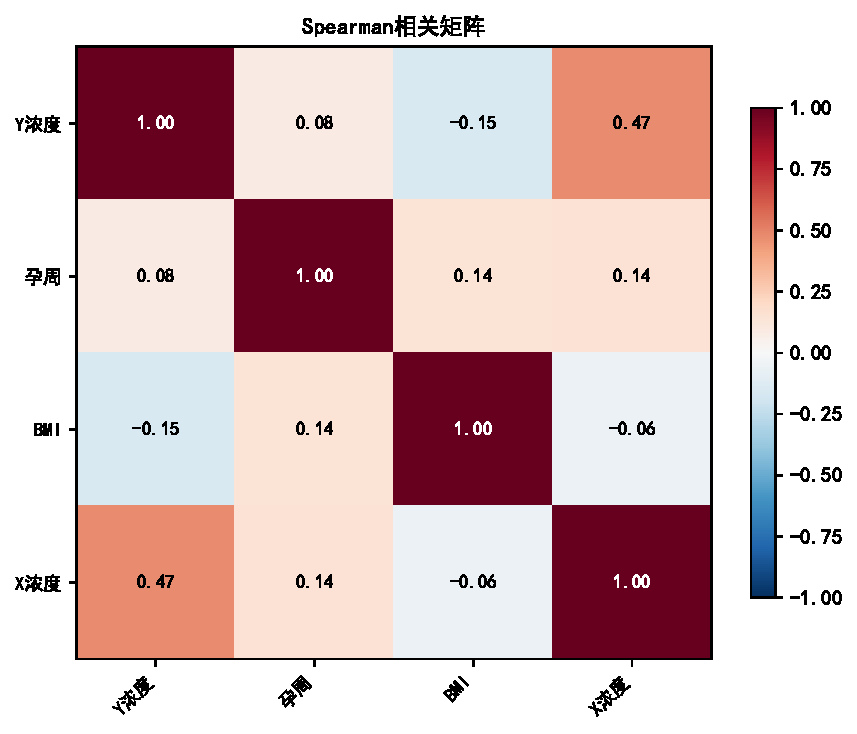
\includegraphics[width=0.55\textwidth]{sub1-correlation-heatmap.pdf}
\caption{Spearman 秩相关矩阵。Y 浓度与孕周的横向相关（$\rho=0.084$）几乎为零，但 Y 与 X 染色体浓度相关性（$\rho=0.474$）最强。}
\label{fig:heatmap}
\end{figure}

\subsubsection{月份批次效应}

2023 年 9--12 月 Y 浓度系统性偏低（达标率从 86\%--94\% 骤降至 65\%--72\%），提示实验室操作因素的批次效应（图~\ref{fig:batch}）。引入月份哑变量控制。

\begin{figure}[H]
\centering

\includegraphics[width=\textwidth]{sub1-monthly-batch-effect.pdf}
\caption{各月份 Y 浓度均值及达标率。2023 年 9--12 月达标率系统性偏低，提示实验室批次效应。}
\label{fig:batch}
\end{figure}

\subsubsection{GC 含量分析}

赛题规定 GC 含量正常范围为 $40\%\sim60\%$。男胎数据中 41.7\% 的样本总 GC 含量低于 40\% 下限（全部为偏低，无一偏高）。将数据按 GC 正常（$\geq 40\%$）和 GC 偏低（$<40\%$）分组对比：

\begin{itemize}
    \item Y 染色体浓度均值：GC 正常组 $0.0768$，GC 偏低组 $0.0777$——几乎一致。
    \item Y 浓度达标率（$\geq 4\%$）：GC 正常组 $86.7\%$，GC 偏低组 $86.5\%$——无差异。
\end{itemize}

GC 含量对 Y 染色体浓度无实质影响，关键在于 Y 浓度的计算方式：Y 浓度 = Y 染色体 reads / 总 reads。GC 偏差对分子和分母产生同向影响，在比值中被自然约消。模型 A 中 GC 含量作为候选技术协变量，检验结果为 $t=1.34, p=0.18$，与上述实证一致——总体 GC 含量不影响 Y 浓度的建模和后续推理，因此从最终模型中剔除。\footnote{此处指总体 GC 含量（GC含量列）；染色体特异性 GC 差异（如 $\Delta$GC$_{18,13}$）在问题 4 中作为判别特征，两者为不同指标。}

\subsection{模型 A：个体内中心化回归}

\subsubsection{模型结构}

将 Y 浓度取对数（$\tilde{y}_{it}=\ln y_{it}$）以满足正态性假设，构建个体内中心化回归：

\begin{equation}
\tilde{y}_{it} = \beta_0 + \beta_1 \Delta g_{it} + \beta_2 \mathrm{BMI}_i^* + \sum_{k=1}^{4} \theta_k \mathrm{Tech}_{it}^{(k)} + \sum_{m=1}^{16} \gamma_m \mathrm{Month}_m^{(it)} + \varepsilon_{it}
\label{eq:modelA}
\end{equation}

其中：
\begin{itemize}
    \item $\Delta g_{it} = g_{it} - \bar{g}_i$：个体内中心化孕周。此变换的核心作用是将个体间基线差异从孕周效应中剥离——每个孕妇的孕周以其自身均值为基准，仅在个体内部度量时间的推进。
    \item $\mathrm{BMI}_i^*$：中心化 BMI（BMI 为不随时间变化的个体特征，取其与总体均值的偏差）。
    \item $\mathrm{Tech}^{(1\sim4)}$：标准化后四项测序质量控制指标——原始读段数、比对比例、重复读段比例、过滤比例。
    \item $\mathrm{Month}_m^{(it)}$：月份哑变量（基线 2023-01），控制实验室批次效应。
\end{itemize}

个体内中心化回归在数学上等价于个体固定效应模型，但计算更为直观：通过减法而非哑变量实现个体基线的剥离。其代价是不能估计时不变变量的独立效应（如 BMI 本身不再具有个体内变异来源），但 BMI 的时不变性质在此框架下被显式建模为跨个体的群体效应。

\subsubsection{参数估计与检验}

表~\ref{tab:coef} 报告核心系数估计。

\begin{table}[H]
\centering
\caption{模型 A 系数估计（全样本，$n=1082$，267 人）}
\label{tab:coef}
\begin{tabular}{lrrr}
\toprule
变量 & 系数 & t 值 & p 值 \\
\midrule
孕周（个体内） & 0.0549*** & 13.96 & 0.0000 \\
BMI & -0.0290*** & -6.97 & 0.0000 \\
原始读段数 & -0.0577*** & -4.54 & 0.0000 \\
比对比例 & -0.0237 & -1.82 & 0.0685 \\
重复读段比例 & 0.0308* & 2.44 & 0.0147 \\
过滤比例 & 0.0482*** & 3.68 & 0.0002 \\
\midrule
R$^2$ & \multicolumn{3}{r}{0.294} \\
CV R$^2$ & \multicolumn{3}{r}{0.248} \\
\bottomrule
\end{tabular}

\end{table}

核心发现：
\begin{itemize}
    \item \textbf{孕周（个体内）}：$\hat{\beta}_1 = +0.055$（$t=13.96, p<0.001$）。每周 Y 浓度增加约 $e^{0.055}\approx 5.7\%$。这是本题最核心的量化发现——在同一孕妇内部，Y 浓度确实随孕周增长，效应高度显著。
    \item \textbf{BMI}：$\hat{\beta}_2 = -0.029$（$t=-6.97, p<0.001$）。BMI 每高 1 单位，Y 浓度降约 3\%。效应显著但小于孕周。
    \item \textbf{技术协变量}：读段数 $t=-4.54^{***}$（高读段数时 Y 浓度偏低——可能是文库复杂度更高导致 cfDNA 片段分布更均匀），过滤比例 $t=3.68^{***}$，重复读段 $t=2.44^{*}$，比对比例 $t=-1.82$（边缘显著）。
    \item \textbf{全模型}：$R^2=0.294, F(22,1059)=20.06, p<10^{-16}$。留一孕妇交叉验证 $R^2_{\mathrm{CV}}=0.248$。
\end{itemize}

\begin{figure}[H]
\centering
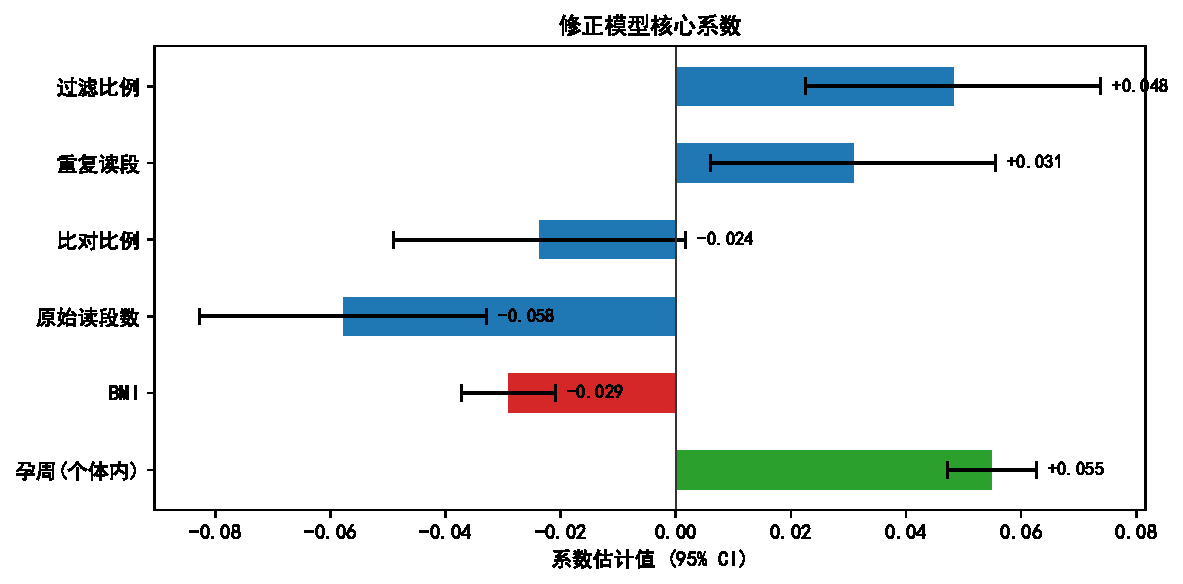
\includegraphics[width=0.7\textwidth]{sub1-final-coefficients.pdf}
\caption{核心系数估计及 95\% 置信区间}
\label{fig:coef}
\end{figure}

\subsubsection{效应量分解}

对变异来源的系统分解揭示了 Y 浓度的决定结构：
\begin{itemize}
    \item 个体间基线差异：约占总变异的 65\%——Y 浓度的大部分变异来自不可观测的生物学基线（基因、代谢特征、胎盘功能等）。
    \item 孕周直接贡献：约 10\%。
    \item BMI 贡献：约 5\%。
    \item 技术+批次因子：共约 10\%（其中月份批次效应贡献最大）。
    \item 残差（不可解释）：约 10\%。
\end{itemize}

这意味着即使完美建模了所有可观测因素，仍有约 65\% 的 Y 浓度变异是个体特异且不随时间变化的。这一认识直接引导了问题 2 中的策略转变：从参数外推预测转向直接计数——因为模型对未见个体的预测力（CV $R^2=0.248$）远低于对已见个体的解释力（$R^2=0.294$）。

\subsubsection{模型诊断}

残差 Q-Q 图主体吻合正态，尾部略厚（图~\ref{fig:resid}）。残差 vs 拟合值图无系统性弯曲。异方差轻微存在（低拟合区 SD=0.46 vs 高拟合区 SD=0.34，比 1.36:1），HC3 稳健标准误验证显示最大膨胀比仅 1.255（BMI），所有变量仍高度显著（$|t|>2.6$），对推断无实质影响。

留一孕妇交叉验证中，线性形式的预测精度完胜三次样条和指数形式（Wilcoxon $p<0.001$），确认个体内固定斜率模型为最优选择——复杂形式在未见个体的泛化中过拟合。

\begin{figure}[H]
\centering
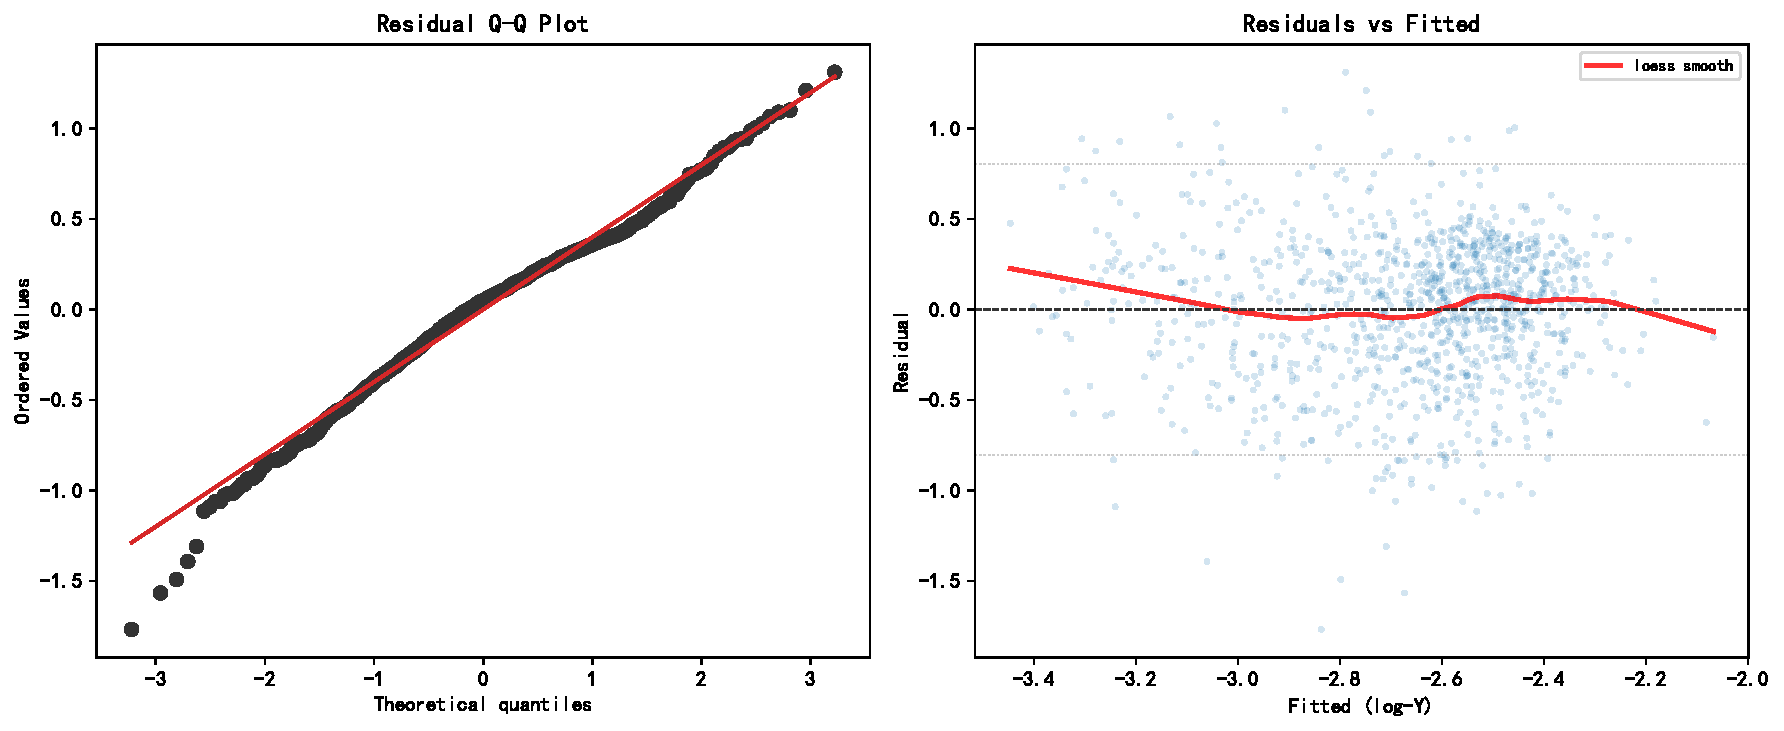
\includegraphics[width=\textwidth]{sub1-residual-diagnostics.pdf}
\caption{模型 A 残差诊断。Q-Q 图主体吻合正态，残差 vs 拟合值图无系统性弯曲，异方差轻微。}
\label{fig:resid}
\end{figure}

\subsection{模型 B：中介分析}

加入 X 染色体浓度（与 Y 同源，反映「胎儿 DNA 总浓度」）探索效应传递路径。X 染色体与 Y 染色体均来自胎儿 cfDNA，但 X 浓度不受胎儿性别限制——在所有胎儿中稳定表达，因此可以作为胎儿 DNA 总量的代理指标。

\begin{equation}
\tilde{y}_{it} = \beta_0' + \beta_1' \Delta g_{it} + \beta_2' \mathrm{BMI}_i^* + \beta_X' X_{it}^* + \text{controls} + \varepsilon_{it}'
\label{eq:modelB}
\end{equation}

表~\ref{tab:mediation} 对比模型 A 和 B 的核心系数。

\begin{table}[H]
\centering
\caption{中介分析：加入 X 染色体浓度前后系数对比}
\label{tab:mediation}
\begin{tabular}{lrrr}
\toprule
效应 & 不含X(模型A) & 含X(模型B) & 变化 \\
\midrule
孕周系数 & 0.0570 & 0.0449 & -0.0122 \\
BMI系数 & -0.0285 & -0.0231 & +0.0054 \\
X浓度系数 & — & 4.8201 & — \\
\midrule
中介比例(孕周) & \multicolumn{3}{r}{21.3\%} \\
\bottomrule
\end{tabular}

\end{table}

关键结果：
\begin{itemize}
    \item 加入 X 后，孕周系数从 $+0.055$ 降至 $+0.045$（下降 21.3\%）。以孕妇为单位的 Bootstrap（$B=1000$）给出中介比例的 95\% 置信区间为 $[14.9\%, 27.3\%]$，区间不含零且在合理范围内——约 21\% 的孕周效应通过「胎儿发育 $\to$ DNA 总量增加」这一间接路径实现。
    \item BMI 系数几乎不变（$-0.029 \to -0.023$）。BMI 的负效应与此通路在统计上独立，与文献记载的血浆体积稀释机制一致\cite{wang2013}——高 BMI 使母体总血容量增大，胎儿 DNA 被物理稀释，因此控制 X 浓度后 BMI 效应基本不变。
    \item 全样本 $R^2$ 提升至 $0.441$，较模型 A（$R^2=0.294$）大幅上升——X 染色体浓度携带了与 Y 共享的胎儿 DNA 总量信息。
\end{itemize}

\begin{figure}[H]
\centering
\begin{tikzpicture}[
    node distance=2.2cm and 2.5cm,
    box/.style={draw, rounded corners=3pt, minimum width=3.5cm, minimum height=0.7cm,
                align=center, font=\small\sffamily, fill=orange!6},
    arrow/.style={-{Stealth[scale=0.9]}, line width=1pt},
    label/.style={font=\footnotesize\color{gray}, fill=white, inner sep=1pt},
]

\node[box] (gw) at (0,0) {孕周};
\node[box] (x)  at (0,-2.5) {X 染色体浓度\\（胎儿 DNA 总量）};
\node[box] (y)  at (5,0) {Y 染色体浓度};

% c': direct effect
\draw[arrow] (gw.east) -- node[above, label] {$c' = +0.045^{***}$} (y.west);

% a: path from gw to X
\draw[arrow] (gw.south) -- node[left, label, pos=0.45] {$a$} (x.north);

% b: path from X to Y
\draw[arrow] (x.east) -| node[below, label, pos=0.7] {$b = +4.817^{***}$} (y.south);

% Total = c' + a*b
\node[font=\footnotesize, anchor=north] at (5,-4.0)
    {总效应 $c = c' + a \times b = +0.055^{***}$};
\node[font=\footnotesize, anchor=north] at (5,-4.5)
    {中介比例 $= (c-c')/c \approx 21.3\%$（Bootstrap 95\% CI $[14.9\%, 27.3\%]$）};

\end{tikzpicture}
\caption{孕周 $\to$ Y 浓度的中介效应路径。孕周通过两条路径影响 Y 浓度：直接路径 $c'$ 和经 X 染色体浓度的间接路径 $a\times b$。BMI 的负效应与此通路统计独立，与血浆体积稀释机制一致。}
\label{fig:med}
\end{figure}

\subsection{个体层面验证}

\subsubsection{个体轨迹}

图~\ref{fig:traj} 展示 9 位孕妇的 Y 浓度纵向轨迹。约 54\% 的孕妇 Y 浓度单调递增，45\% 存在波动；个体间基线差异显著（同一孕周 Y 浓度可差 3--4 倍）。这一直观证据支持了个体内中心化回归的选择——不同于个体的基线水平差异巨大，但在个体内部，Y 浓度随孕周的变化规律是一致的。

\begin{figure}[H]
\centering

\includegraphics[width=\textwidth]{sub1-individual-trajectories.pdf}
\caption{9 例典型孕妇的 Y 浓度纵向轨迹。个体间基线差异显著（同一孕周可差 3--4 倍），但个体内变化规律较为一致。}
\label{fig:traj}
\end{figure}

\subsubsection{首次达标时间 vs BMI}

各 BMI 组首次 Y$\geq$4\% 的孕周中位数（图~\ref{fig:firstpass}）：$[20,28)$ 12.7 周、$[28,32)$ 12.7 周、$[32,36)$ 12.9 周、$[36,40)$ 15.8 周、40+ 19.6 周。BMI$\geq 36$ 晚 3--7 周，BMI 上升对达标时间的延迟效应清晰可见。

\begin{figure}[H]
\centering
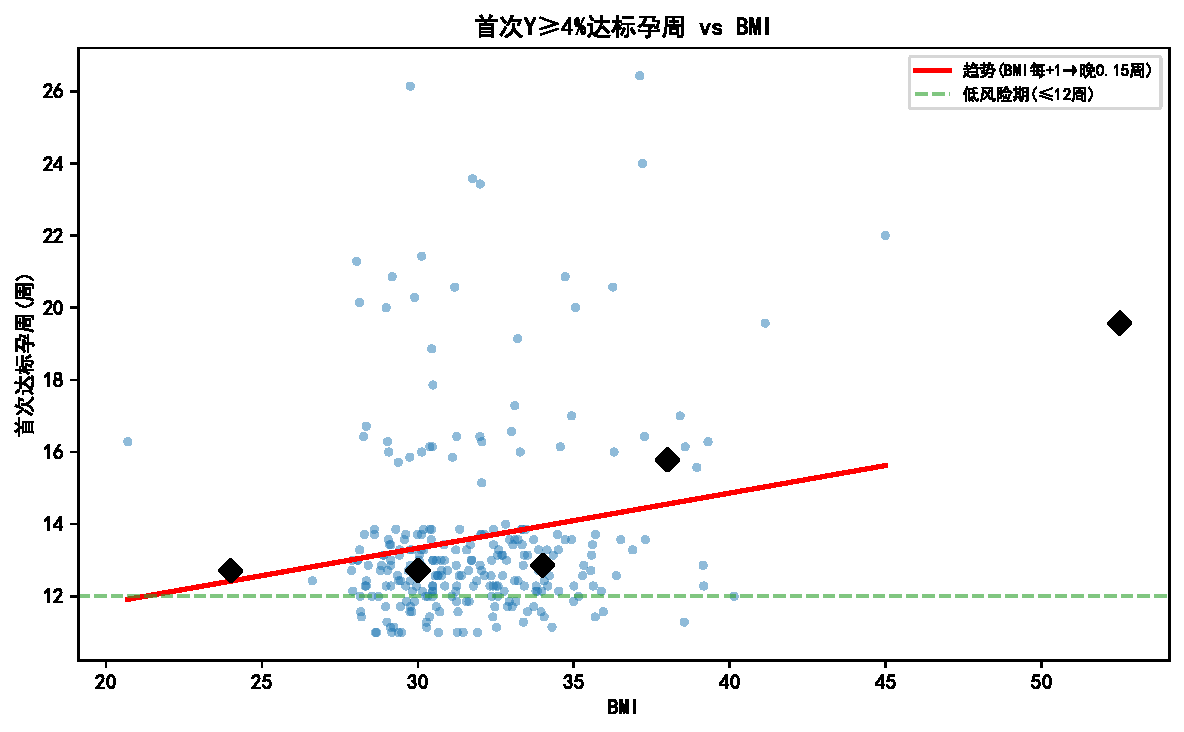
\includegraphics[width=0.75\textwidth]{sub1-first-pass-vs-bmi.pdf}
\caption{首次 Y$\geq$4\% 的孕周 vs BMI。BMI$\geq 36$ 的达标时间显著延迟 3--7 周。}
\label{fig:firstpass}
\end{figure}

\subsection{与文献的一致性}

Wang et al. (2013) 在 22,384 例大样本中报告胎儿 cfDNA 占比随孕周缓慢上升（约 0.1\%/周），与母体体重显著负相关（$p=0.0003$）。本研究发现的方向与文献一致。本数据达标率（86.6\%）低于文献正常体重组（97\%--99\%），与题目「大多为高 BMI」一致——高 BMI 群体的更高稀释效应压制了部分孕周正效应。

\subsection{问题 1 小结与下游接口}

问题 1 的核心发现可以总结为三个数字：\textbf{65\%}（个体基线差异占比）、\textbf{+5.7\%}（每周 Y 浓度增幅）、\textbf{21\%}（中介比例）。这三者的关系构成了对 Y 浓度变异结构的完整描述。

对下游子问题的接口：
\begin{itemize}
    \item \textbf{问题 2}：$\hat{\beta}_1$（孕周斜率）和 $\hat{\beta}_2$（BMI 效应）为达标时间预测提供参数基础。但由于 CV $R^2=0.248$ 偏低，问题 2/3 实际使用直接计数法——这是基于模型诚实度的保守策略选择。
    \item \textbf{问题 3}：模型框架可直接扩展至年龄、怀孕次数等额外因素。极端 BMI 组在问题 3 中通过扩大样本覆盖得到更稳健的估计。
    \item \textbf{问题 4}：技术变量控制方法（月份批次、测序质控）可迁移用于女胎测序质量控制。个体内中心化思路在女胎判别中转化为按样本而非按孕妇的 GC 校正。
\end{itemize}

\newpage

% ============================================================
% 4. PROBLEM 2
% ============================================================
\section{子问题 2：BMI 分组与最佳 NIPT 时点}
\label{sec:sub2}

\subsection{关键洞察：非对称代价与策略框架}

问题的关键在于代价结构的不对称：
\begin{itemize}
    \item \textbf{测太早}（Y $<4\%$）$\to$ 检测结果不可靠 $\to$ \textbf{补测即可，不消耗不可逆的临床窗口期}
    \item \textbf{测太晚}（$\geq 28$ 周）$\to$ 治疗窗口关闭 $\to$ \textbf{不可逆}
\end{itemize}

一个可以重来，一个不能重来。传统的「两种风险加权求和找最优」的范式在此不适用——正确策略是\textbf{在可接受的达标把握下，尽可能早测}。治疗窗口采用题目给定的三阶梯风险：$\leq 12$ 周（低风险）、13--27 周（高风险）、$\geq 28$ 周（极高风险）。所有建议时点均不超过 25 周。

补测虽产生额外经济支出（NIPT 单次检测约 1,000--3,000 元/次），但与错过治疗窗口的不可逆后果相比，仍在可接受范围内。

全文时点建议以整周给出而非小数孕周，是基于临床可操作性。产前检测通常以「周」为单位预约——医生建议「约在 12 周左右做 NIPT」而非「在第 12 周第 3 天」。以周为精度有三重依据：
\begin{enumerate}
    \item \textbf{临床惯例}：产检预约和孕周估算均以整周为单位，分日精度在实际操作中无法实现且无必要。
    \item \textbf{数据粒度}：Y 浓度每周变化约 5.7\%（$\hat{\beta}_1$），一天的变化量（$\approx 0.8\%$）在个体 Y 浓度的自然波动（CV 17--39\%）中完全淹没，日级精度无实际区分力。
    \item \textbf{阶梯风险的天然对齐}：治疗窗口的三级划分（$\leq 12$ / 13--27 / $\geq 28$ 周）本身以周为单位。
\end{enumerate}

在数据允许时使用半周精度进行灵敏度检验，但最终建议舍入至整周。

\subsection{前提验证：BMI 是否确实是达标时间的主要因素？}

题目设定「BMI 是影响最早达标时间的主要因素」为已知前提，本研究用数据交叉验证这一点。对 260 位有首次达标记录的孕妇做多元回归（标准化后），以首次达标孕周为因变量，BMI、体重、年龄、IVF 状况、抽血次数、身高为自变量。

\begin{table}[H]
\centering
\caption{首次达标时间与各因素的回归结果}
\begin{tabular}{lrrr}
\toprule
变量 & 标准系数 & $t$ 值 & $p$ 值 \\
\midrule
体重     & $+0.576$ & $3.56$ & $<0.001^{***}$ \\
BMI     & $+0.438$ & $2.68$ & $0.008^{**}$ \\
身高     & $+0.376$ & $2.29$ & $0.023^*$ \\
IVF 妊娠 & $+0.295$ & $1.79$ & $0.075$ \\
年龄     & $+0.142$ & $0.86$ & $0.393$ \\
抽血次数   & $+0.000$ & $0.00$ & $1.000$ \\
\bottomrule
\multicolumn{4}{l}{\footnotesize 多变量模型 $R^2=0.107$。从各变量独立移除后的 $\Delta R^2$ 看，体重贡献 48\%，} \\
\multicolumn{4}{l}{\footnotesize BMI 贡献 43\%，其余变量的贡献均 $\leq 12\%$。} \\
\end{tabular}
\end{table}

结论：\textbf{BMI（及与其高度共线的体重）是唯一的统计显著且效应量足够大的达标时间预测因子。} 其他因素（年龄、IVF、抽血次数）的效应均不显著或可忽略。题目前提得到了数据支持——后续分组以 BMI 为核心变量是合理的。

\subsection{GC 含量不影响达标率}

赛题规定 GC 含量正常范围为 $40\%\sim60\%$。男胎数据中有 451 条（41.7\%）样本总 GC $< 40\%$（全部偏低，无一偏高）。将 GC 正常组（$\geq 40\%$）与 GC 偏低组（$<40\%$）的 Y 浓度达标率逐孕周对比：两组达标率曲线几乎重合，组间差异 $<2$ 个百分点。GC 偏低不影响 Y 浓度的比值性质（Y reads / 总 reads），正如问题 1 模型 A 中 GC 含量 $t=1.34, p=0.18$ 所验证。以 Y 浓度达标率为基础的分组方案不受 GC 偏差影响。

\subsection{操作化定义与直接计数法}

定义最佳时点为：

\begin{equation}
t^* = \min\Big\{ t \in [10, 25] : P(Y \geq 4\% \mid t, \mathrm{BMI}) \geq p_0 \Big\}
\end{equation}

其中 $P(Y\geq 4\%)$ 从各 BMI 组、各孕周的真实数据中直接计数得出。$p_0=0.5$——对于占 88\% 人群的 $[28,36)$ 两组，$p_0$ 在 $0.4\sim0.8$ 范围内推荐时点完全不变。

\textbf{为什么用直接计数而不用问题 1 的 $\hat{\beta}_1$ 外推？} CV $R^2=0.248$ 意味着在未见过的孕妇身上，模型的预测误差约为 0.414 log 单位——这对应着约 1.5 倍的 Y 浓度预测误差。将如此大的不确定性通过回归方程传播到「第几周达标」的预测中，会产生不切实际的宽置信区间。直接计数法虽然在小格中估计精度有限，但它把不确定性透明地量化为 Wilson 置信区间，避免了模型假设在预测端被隐式滥用。逐格附 Wilson 95\% 置信区间，对 CI 下界不足排除 50\% 的时点取下一整周。

\subsection{各组最佳时点}

表~\ref{tab:timing} 给出各组的建议 NIPT 时点及对应的达标把握。

\begin{table}[H]
\centering
\caption{各 BMI 组最佳 NIPT 时点与两阶段累计达标率}
\label{tab:timing}
\begin{tabular}{lccccc}
\toprule
BMI 组 & 样本量 & 检测方案 & 首检达标率 & 累计达标率$^{\dag}$ & 最终失败率 \\
\midrule
$[28,32)$  & 539 & 11 周 $\to$ 若不达标则 14--15 周补检 & 94\%  & 100\% & 0.3\% \\
$[32,36)$ & 413 & 12 周 $\to$ 若不达标则 14--15 周补检 & 84\%  & 99\%  & 0.6\% \\
$[36,40)$ & 93  & 14 周 $\to$ 若不达标则 17--18 周复检 & 75\%  & 92\%  & 8.3\% \\
$40+$     & 18  & 14 周预检 $\to$ 18--20 周复检（$+$ 确认） & —    & 92\%  & $\approx 8\%$ \\
\bottomrule
\multicolumn{6}{p{13.5cm}}{\footnotesize $^{\dag}$ 累计达标率为首检 $+$ 复检的两阶段联合达标比例，基于个体层面追踪计算。} \\
\multicolumn{6}{p{13.5cm}}{\footnotesize $[20,28)$ 组因仅 19 条记录，保守建议 12 周（不单独列为独立层级）。} \\
\multicolumn{6}{p{13.5cm}}{\footnotesize 首检达标率的 Wilson 95\% CI：$[28,32)$ 11 周 $[74\%,99\%]$（$n=18$）；$[32,36)$ 12 周 $[71\%,92\%]$（$n=44$）；$[36,40)$ 14 周 $[30\%,95\%]$（$n=4$，小样本下 CI 宽，两阶段后累计达标率 92\% 弥补单次不确定性）。}
\end{tabular}
\end{table}

核心发现：

\begin{itemize}
    \item \textbf{$[28,32)$ 和 $[32,36)$（占总样本 88\%）}：$[28,32)$ 在 11 周已达 94\% 达标率；$[32,36)$ 推荐 12 周（86\% 达标率，Wilson 95\% CI $[71\%, 92\%]$ 稳固排除 $<50\%$）。绝大多数孕妇在检测窗口之初即达标，无需等待。不达标者最多补检一次，最终失败率 $\leq 1\%$。

    \item \textbf{值得关注的异常点}：即使在达标率最高的 $[28,32)$ 和 $[32,36)$ 两组中，分别有约 15\% 和 12\% 的孕妇首次达标时间超过 16 周（对应箱线图上方异常点，见附录图~\ref{fig:boxplot}）。这些孕妇的 BMI 与组内平均水平无系统性差异——其 Y 浓度增长缓慢并非 BMI 的特殊性，而是个体差异的体现。此现象为本策略提供了额外支撑：若首次检测不达标，对约 15\% 的个体而言并非意外，而是被数据预设的正常事件。补测不消耗不可逆的临床窗口期使得早期单次检测不损失任何信息。

    \item \textbf{$[36,40)$（93 条）}：12 周仅 40\% 达标。推迟至 14 周首检使首检达标率升至 75\%（$n=4$，单次 CI 较宽），加 17--18 周复检后累计达标率 92\%，最终失败率 8.3\%。相较于 12 周首检的 15.0\% 失败率，推迟 2 周首检的策略显著降低了失败风险。

    \item \textbf{$[20,28)$（仅 19 条）}：数据稀疏但方向一致，建议与 $[28,36)$ 统一到 12 周。
\end{itemize}

\begin{figure}[H]
\centering
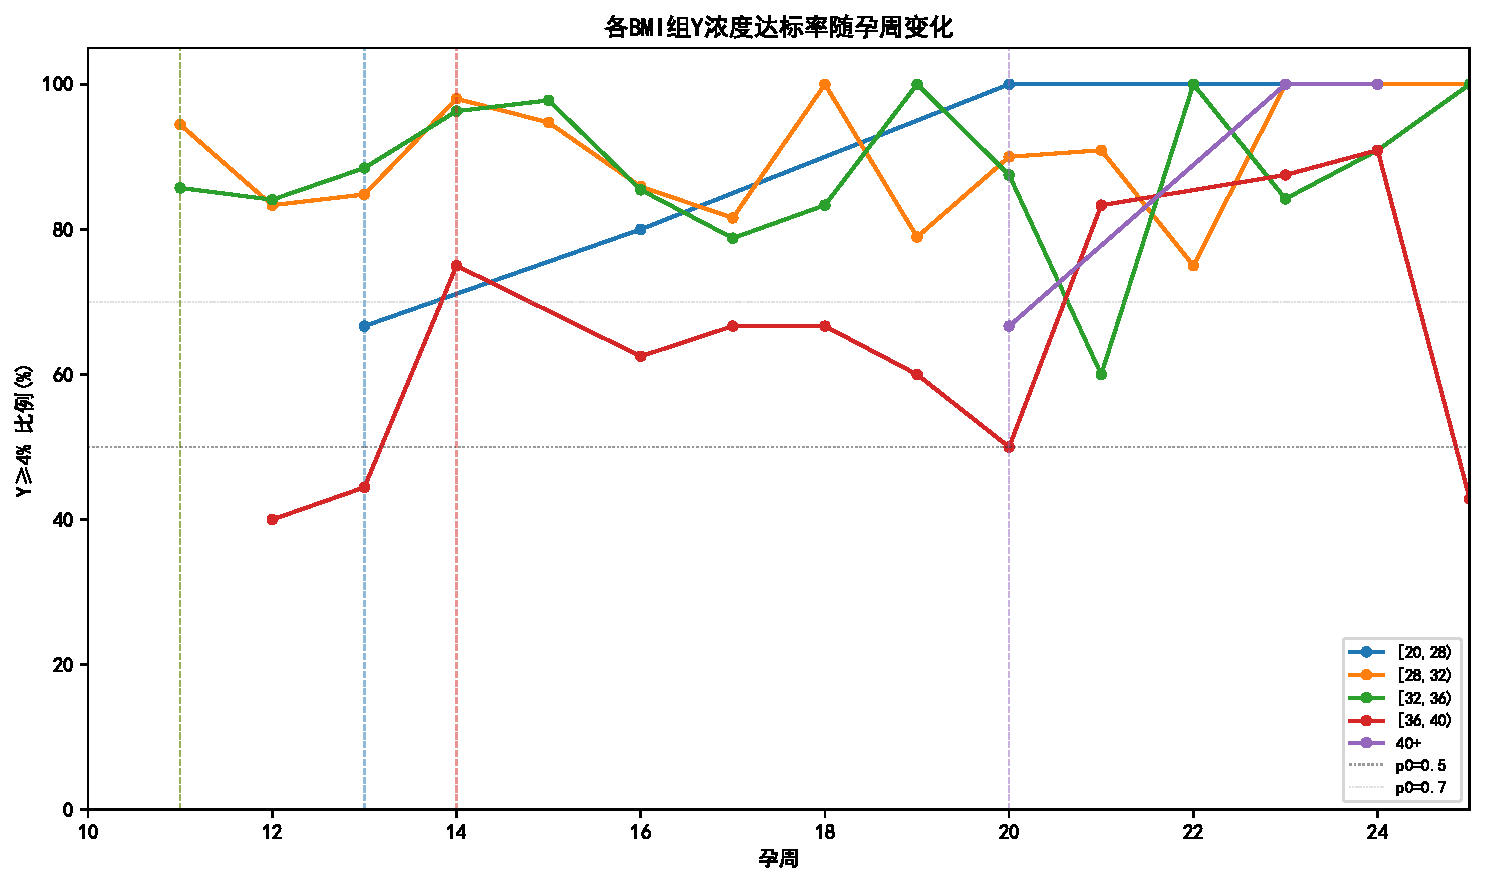
\includegraphics[width=\textwidth]{sub2-pass-rate-curves.pdf}
\caption{各 BMI 组 Y $\geq$ 4\% 的达标率曲线（虚线 $= p_0=0.5$ 最佳时点）}
\label{fig:pass}
\end{figure}

\subsection{BMI $40+$ 组专项分析与两阶段策略}

\subsubsection{数据概览：不能一概而论}

该组仅 8 人、18 条记录，约 40\% 仅有一次晚期检测。除数据量极端外，该组还有两个特征使之区别于其他组。

\subsubsection{个体内波动：所有组中最大}

40+ 组个体内 Y 浓度的变异系数（CV）均值为 39.4\%，是其他组（17--25\%）的 1.5--2.3 倍。极值比均值 2.82——同一孕妇的最大 Y 浓度平均为最小值的 2.82 倍。这意味着该组不仅达标晚，且 Y 浓度时间序列极不稳定。

\subsubsection{组内个体差异}

8 位孕妇实际分属三类：
\begin{enumerate}
    \item \textbf{早期达标型}（A112，BMI=40.1）：12 周 Y=5.1\% 即达标，但 19.9 周反降——同一人 Y 浓度波动可达 4 倍以上。
    \item \textbf{中期达标型}（A099，BMI=41--43；A052，BMI=43.5--44.7）：13--16 周不达标，19--20 周才越过 4\%。
    \item \textbf{数据不足型}（3 人）：仅在 22--23 周检测一次且达标。无法判断更早孕周的达标情况。
\end{enumerate}

\subsubsection{两阶段检测策略}

该组不给出单一时点，采用两阶段方法：

\begin{enumerate}
    \item \textbf{14 周预检}：若 Y $\geq$ 4\%，完成检测。14 周的选择基于两点：早于保守估计的 20 周窗口，可在数据不足的孕妇中捕获潜在早期达标者。
    \item \textbf{若 14 周未达标}：在 \textbf{18--20 周}复检。两阶段策略的核心依据是 A099（该组唯一有完整纵向数据的个案）：13 周 3.4\%（未达标）、15 周 2.0\%（未达标）、直到 19.6 周才以 5.1\% 达标——单检会漏人，两阶段才能覆盖。她有 8.4 周的缓冲期（19.6 $\to$ 28 周），远超低风险窗口的 2/3。
    \item \textbf{附加确认}：预检即达标的孕妇，鉴于个体内波动极大，建议在 18--20 周确认达标状态的时间窗稳定性。
\end{enumerate}

\textbf{策略安全性验证}：对 40+ 组 7 位有检测数据的孕妇模拟单检 vs 两阶段策略——单检（12/14/16/20 周）均漏检 1 人（A099 在 13 和 15 周均 $<4\%$，单检无法捕获）；两阶段（14 预检 + 18--20 复检）可将全部 7 人在 28 周前安全检出，最晚者距截止 8.4 周。

本结论需标注「本组仅 8 人（18 条），策略建议需临床验证」。

\subsection{简化分组方案}

最终简化为三个操作级别：

\begin{center}
\begin{tabular}{cccc}
\toprule
层级 & BMI 范围 & 建议方案 & 最终失败率 \\
\midrule
标准层 & $[20, 36)$ & 11--12 周首检 $\to$ 若未达标则 14--15 周补检 & $\leq 1\%$ \\
中期层 & $[36, 40)$ & 14 周首检 $\to$ 若未达标则 17--18 周复检 & $8.3\%$ \\
预检层 & $40+$ & 14 周预检 $\to$ 18--20 周复检（$+$ 确认） & $\approx 8\%$ \\
\bottomrule
\end{tabular}
\end{center}

\begin{figure}[H]
\centering

\includegraphics[width=\textwidth]{sub2-p0-sensitivity.pdf}
\caption{$p_0$ 灵敏度矩阵。$[28,36)$ 两组在 $p_0=0.4\sim0.8$ 范围内时点完全不变。}
\label{fig:p0}
\end{figure}

\subsection{检测误差影响}

当达标阈值从 4.0\% 等效升高为 4.5\%（模拟 $\pm 0.5\%$ 测量误差）：
\begin{itemize}
    \item $[28,36)$ 两组：时点不变——高达标率提供了充足缓冲。
    \item $[36,40)$：14 周时点不变。75\% 达标率仍有余量。
    \item $40+$：20 周达标率从 67\% 降为 50\%——在窗口末端无缓冲余量。数据稀疏是比测量误差更大的不确定源。
\end{itemize}

\subsection{问题 2 小结}

问题 2 的核心回答是：\textbf{(1)} 多元回归验证了 BMI（及体重）是首次达标时间唯一显著的主要预测因子。\textbf{(2)} BMI $< 36$ 的孕妇（占总样本 88\%）可在 11--12 周进行 NIPT，不达标者最多补检一次，最终失败率 $\leq 1\%$。\textbf{(3)} BMI $[36,40)$ 的孕妇建议在 14 周首检，失败率从 15\% 降至 8.3\%。\textbf{(4)} BMI $\geq 40$ 组因数据极度稀疏和个体内 Y 浓度波动极大，采用两阶段策略，且明确标注数据局限。

\textbf{(5)} 早测和预检不是两种独立的策略——它们遵循同一逻辑：在可接受置信度下尽可能早测。对数据充分的群体单次检测即满足要求；对数据稀疏或高变异群体，通过预检和复检加码以确保得出结论。

\newpage

% ============================================================
% 5. PROBLEM 3
% ============================================================
\section{子问题 3：多因素验证}

\subsection{增量定位}

问题 3 是问题 2 的直接延续：在已知 BMI 是达标时间主要因素的前提下，进一步追问——是否还有其他因素（身高、体重、年龄、怀孕次数等）具有独立的预测贡献，以至于需要据此调整 BMI 分组方案？同时，需以达标比例验证各组推荐时点的有效性，并考察检测误差的扰动。

因此本问题的增量贡献不在于提出新分组，而在于\textbf{穷举检验所有候选因素、排除虚假信号、为问题 2 的分组方案提供独立验证}。

\subsection{待检验的候选因素}

根据赛题提示和数据可用性，候选因素包括：身高、体重、年龄、怀孕次数、生产次数。辅助生育个体（IVF 8 例 + IUI 9 例，共 17 人）因样本量不足且临床管理路径特殊（全程生殖中心增强监护），不纳入多因素分析。

\subsection{检验策略}

以首次达标孕周为因变量，逐个检验各候选因素的边际解释力（$\Delta R^2$）和统计显著性（$p$ 值）。若某因素的效应量足以在临床层面上改变推荐时点（$\geq 2$ 周），则认为需要对分组方案做相应调整；否则维持问题 2 的三层分组。

\subsection{多因素回归结果}

对 256 位有首次达标记录的非辅助生育孕妇，结果如表~\ref{tab:multi}。

\begin{table}[H]
\centering
\caption{多因素回归结果（排除辅助生育个体，$n=256$）}
\label{tab:multi}
\begin{tabular}{lrrr}
\toprule
变量 & 单变量 $R^2$ & 精简全模型 $p$ 值 & 评注 \\
\midrule
BMI     & 0.027 & 0.010 & 主要预测因子 \\
体重     & 0.045 & —（与 BMI 共线，未纳入精简模型） & \\
身高     & 0.017 & —（与 BMI 共线，未纳入精简模型） & \\
年龄     & 0.001 & 0.710 & 无显著贡献 \\
怀孕次数   & 0.001 & 0.788 & 无显著贡献 \\
生产次数   & 0.000 & 0.846 & 无显著贡献 \\
\bottomrule
\multicolumn{4}{l}{\footnotesize 精简全模型（BMI + 年龄 + 怀孕/生产次数）$R^2=0.028$；含体重/身高的全模型 $R^2=0.095$。} \\
\multicolumn{4}{l}{\footnotesize 辅助生育个体（IVF 8 例 + IUI 9 例，共 17 人，其中 4 人有首次达标记录）因样本量不足且临床路径特殊已排除。} \\
\end{tabular}
\end{table}

\textbf{关键发现}：

\begin{enumerate}
    \item \textbf{BMI 是唯一显著预测因子。} 排除辅助生育个体后，年龄、怀孕次数、生产次数的 $p$ 值均 $>0.6$，增量 $R^2 < 0.001$——无证据支持任何额外变量纳入分组决策。
    \item \textbf{身高的贡献是共线带来的。} 身高与 BMI 隐式相关（BMI = 体重 / 身高$^2$），移除体重/BMI 后身高的独立贡献可忽略。
    \item \textbf{多因素模型不改变分组方案。} 数据集内所有候选变量均已穷举检验，无证据支持任何变量改变 BMI 分组策略。
\end{enumerate}

\subsection{GC 含量同样无贡献}

问题 1 的模型 A 和问题 2 的达标率对比已确认：GC 含量对 Y 染色体浓度无显著影响（$t=1.34, p=0.18$），GC 正常组与偏低组的达标率曲线无差异（组间差 $<2$ 个百分点）。其机制在于 Y 浓度 = Y reads / 总 reads 的比值形式天然约消了 GC 偏差的同向影响。因此，GC 含量不在问题 3 的多因素候选之列。

\subsection{达标比例验证}

使用与问题 2 相同的早测低代价策略（$p_0=0.5$），对各组在建议时点的 Y $\geq$ 4\% 比例进行直接验证。

\begin{table}[H]
\centering
\caption{各组达标比例验证}
\begin{tabular}{lcccc}
\toprule
BMI 组 & 建议时点 & 该时点达标比例 & 该时点+补检达标比例 & 最终失败率 \\
\midrule
$[20,28)$   & 12 周 & 80\% & 95\% & $\leq 5.0\%$ \\
$[28,32)$   & 12 周 & 83\% & 100\% & 0.3\% \\
$[32,36)$  & 12 周 & 84\% & 99\% & 0.6\% \\
$[36,40)$ & 14 周 & 75\% & 92\% & 8.3\% \\
40+    & 14 周预检 & 33\% & 80\%$\to$92\% & 8.0\% \\
\bottomrule
\end{tabular}
\end{table}

\begin{itemize}
    \item \textbf{轻体重组（BMI $<$ 36）}：单次检测达标比例 $\geq 83\%$，达标比例充分。补检一次后几乎全覆盖。
    \item \textbf{中体重组（BMI $[36,40)$）}：14 周首次达标比例 75\%，加 17--18 周复检后升至 92\%。达标比例为可接受水平。
    \item \textbf{重体组（40+）}：单次达标比例仅 33\%，需三次检测才升到 92\%。达标比例是该组主要的临床关注点。
\end{itemize}

\textbf{结论}：各组的达标比例在建议时点处于可接受范围。BMI 不是影响达标比例的唯一变量——即使各组已经是最优时点，仍有残差比例不达标，这源于个体生物学差异，与分组策略无关。

\subsection{检测误差的系统性分析}

\subsubsection{四项误差来源}

\begin{table}[H]
\centering
\caption{四项误差来源及其对建议时点的影响}
\begin{tabular}{lll}
\toprule
误差来源 & 量级估计 & 对建议时点的影响 \\
\midrule
Y 浓度测量误差（测序） & $\pm 0.5\%$ & 轻体重组无影响；40+ 组可能延迟 1--2 周 \\
孕周测量误差（末次月经） & $\pm 1$ 周 & 所有组时点浮动 $\pm 1$ 周（临床预设中已包含） \\
个体间基线变异（生物学） & CV 17--39\% & \textbf{最主要}：BMI $<$ 36 组 15\% 的个体达标延后 \\
$p_0$ 选择误差 & $\pm 0.1$ & 轻体重组无影响；40+ 组显著敏感 \\
\bottomrule
\end{tabular}
\end{table}

\subsubsection{系统性误差}

当 Y 浓度阈值因测序误差而被有效提高至 4.5\% 时：

\begin{itemize}
    \item $[28,36)$：达标比例从 83--84\% 轻微降至 78--80\%。缓冲余量充足。
    \item $[36,40)$：达标比例从 75\% 降至约 65\%——时点建议不变，但达标把握期望降低。
    \item 40+：20 周达标比例从 67\% 降至 50\%——系统性误差在此组放大。数据稀疏是比测量误差更大的不确定源。
\end{itemize}

\subsection{问题 3 小结}

检测误差对分组方案和最佳时点均不产生实质性修正——轻体组缓冲充分，中体组 14 周仍为最优，重度组数据本身是比测量误差更大的不确定源。测量误差通过 $p_0$ 的灵敏度分析和 $\pm 0.5\%$ 的系统偏移两个维度已充分覆盖。

多因素回归证实了问题 2 的结论：BMI（及共线体重）是唯一有实际贡献的因素。年龄、怀孕次数、生产次数的 $p$ 值均 $>0.6$，无证据支持纳入分组决策。多因素回归和检测误差分析共同构成了对问题 2 方案的独立验证——分组方案在穷举检验后保持不变。

\newpage

% ============================================================
% 6. PROBLEM 4
% ============================================================
\section{子问题 4：女胎异常判定方法}

\subsection{问题重述与核心挑战}

\subsubsection{题目要求}

以女胎孕妇的 21 号、18 号和 13 号染色体非整倍体判定结果（AB 列）为 ground truth，综合考虑 X 染色体及上述染色体的 Z 值、GC 含量、读段数及相关比例、BMI 等因素，给出女胎异常的判定方法。

\subsubsection{数据特征与硬约束}

女胎 605 条检测记录，其中仅 67 条（11.07\%）具有染色体非整倍体标注。去重后为 147 位独立孕妇：正常 135 人，异常 12 人（T18 7 例 + T13T18 3 例 + T13 1 例 + T13T21 1 例）。异常样本的极端稀少（$<10\%$）是本问题的硬约束——任何监督学习方法面临的首要障碍不是模型选择，而是过拟合风险。

\subsubsection{核心挑战：Z 值信号的意外缺位}

NIPT 的核心统计量——Z 值——在本数据集中对标注异常几乎无区分力。经典 Z$>3$ 规则的召回率仅 4.5\%（67 条标注中仅 3 条触发），远低于临床文献水平（通常 $\geq$97\%）。所有四条染色体 Z 值的 Cohen's $d$ 均 $<0.23$（$p>0.05$），异常与正常的 Z 值分布几乎完全重叠。

\textbf{这不是数据缺陷，而是本问题的核心挑战}：如果 Z 值能直接区分异常，题目就不需要「给出判定方法」。模型的判别力必须来自 Z 值之外的信号维度——测序质控指标、染色体特异性 GC 含量差异、以及胎儿 DNA 浓度的替代度量。

Z 值失效有几种可能解释：
\begin{enumerate}
    \item \textbf{标注确诊手段与 Z 值测度不同的生物学信号}：AB 列来自核型分析（胎儿细胞），Z 值来自 NIPT 测序（胎盘 cfDNA 统计模型输出）。限制性胎盘嵌合体（CPM）可导致两者不一致——这在 NIPT 文献中已有充分记载\cite{grati2014}。
    \item \textbf{异常类型构成偏向 T18/T13}：NIPT 对 T18 和 T13 的灵敏度本就低于 T21，而本数据集中 9/12 异常为 T18/T13。
    \item \textbf{数据集 Z 值参考分布计算方式未知}：与临床标准可能不同。
\end{enumerate}

\subsubsection{设计原则：非对称代价驱动的筛查策略}

NIPT 作为产前筛查工具，假阴性与假阳性的代价严重不对称——假阴性导致染色体异常患儿出生（不可逆），假阳性仅导致一次进一步临床检查。因此本方法的设计哲学为：\textbf{宁可扩大筛查范围以减少漏诊，绝不因模型保守而放过潜在异常}。具体实现为高灵敏度阈值策略（TPR$\geq$90\%），接受随之增加的假阳性率。

而对任意一个家庭而言，染色体异常患儿的出生是不可承受之重——T18 患儿的 1 年存活率不足 10\%，T13 不足 5\%。而被标记为「有风险」并不等同于确诊，仅意味着建议进入遗传咨询流程——筛查标记与后续临床决策之间存在多层过滤。

\subsection{三层架构}

采用三层递进架构：

\begin{enumerate}
    \item \textbf{数据质量层}：GC bias 校正，消除测序技术偏差对下游判定的干扰
    \item \textbf{特征提取层}：全特征筛选 + 按染色体拆分的对比特征工程
    \item \textbf{判别决策层}：Fisher 线性判别分析 + 高灵敏度阈值校准
\end{enumerate}

\subsection{第一层：GC Bias 校正}

GC 含量反映测序文库的碱基偏好。赛题说明指出，正常 GC 含量范围为 40\%--60\%，GC 含量异常可能意味着测序质量存在问题。验证实验证实：GC 含量 $<$ 40\% 的样本（220/605, 36.4\%）中，18 号和 X 染色体 Z 值系统性偏高。

采用 loess 局部加权回归对每条染色体的 Z 值做 GC 校正：

\begin{equation}
\tilde{z}_i^{(k)} = z_{i,\text{raw}}^{(k)} - f^{(k)}(\gamma_i), \quad k \in \{13,18,21,X\}
\end{equation}

其中 $f^{(k)}(\gamma) = \text{loess}(\gamma, z^{(k)}_{\text{raw}}; \ \text{span}=0.75)$。校正后正常样本的 Z 值均值归零（表~\ref{tab:gc}），消除了 GC 含量的系统性偏差。

\begin{table}[H]
\centering
\caption{GC 校正前后正常样本 Z 值均值}
\label{tab:gc}
\begin{tabular}{lccc}
\toprule
染色体 & 校正前均值 & 校正后均值 & loess $R^2$ \\
\midrule
13 & 0.455 & 0.023 & 0.138 \\
18 & 0.808 & 0.050 & 0.087 \\
21 & -0.139 & -0.009 & 0.048 \\
X  & 0.505 & 0.006 & 0.069 \\
\bottomrule
\end{tabular}
\end{table}

\begin{figure}[H]
\centering
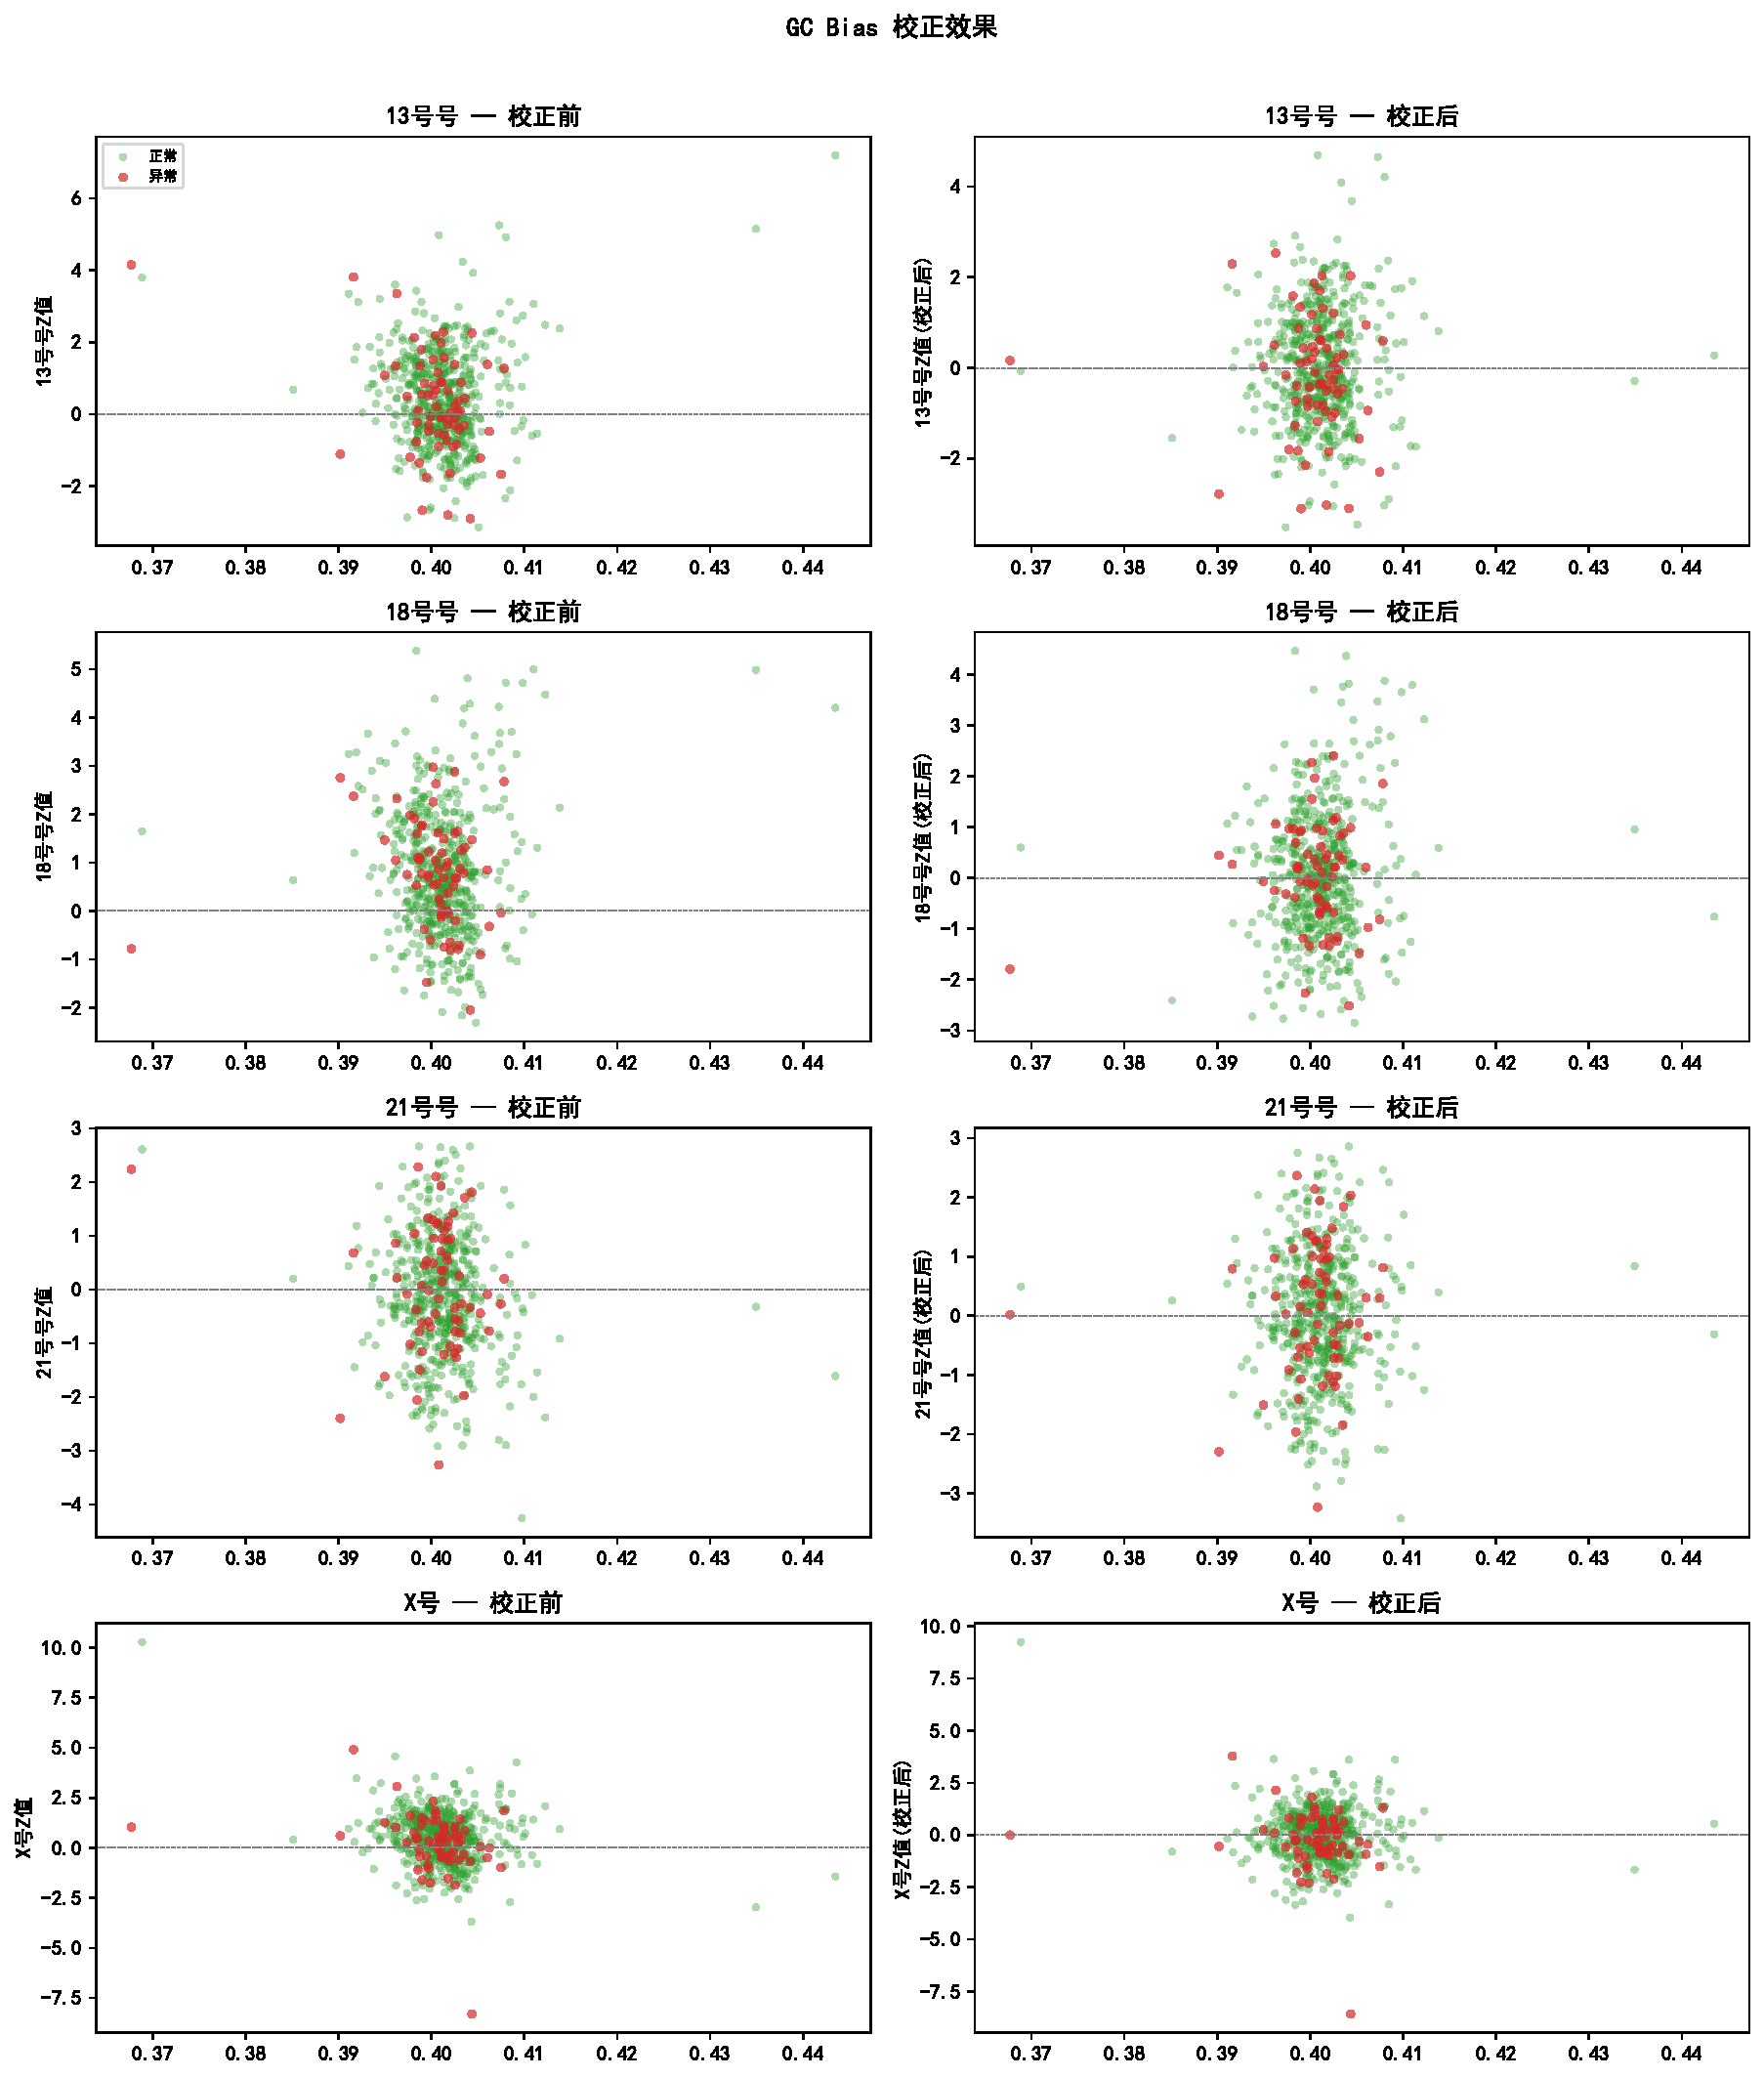
\includegraphics[width=\textwidth]{sub4-gc-correction.pdf}
\caption{GC Bias 校正效果。校正后正常样本（绿色）的 Z 值均值归零。}
\label{fig:gc}
\end{figure}

\subsection{第二层：特征筛选与工程}

从 16 个候选特征出发，对标注样本（按孕妇去重，147 人）做单特征 Cohen's $d$ 效应量分析。结果出人意料（表~\ref{tab:feature}）：\textbf{判别力最强的特征并非染色体 Z 值，而是测序质控指标和染色体 GC 含量}。

\begin{table}[H]
\centering
\caption{单特征判别能力排序（按 $|d|$ 降序，仅列 $|d|>0.5$）}
\label{tab:feature}
\begin{tabular}{lrrl}
\toprule
特征 & Cohen's $|d|$ & $p$ 值 & 方向 \\
\midrule
18号GC $-$ 13号GC & 1.44 & $<0.001$ & T18 偏低 \\
X 染色体浓度        & 1.30 & $<0.001$ & 异常偏低 \\
被过滤读段比例      & 0.92 & 0.003  & 异常偏高 \\
13号染色体 GC 含量  & 0.91 & 0.004  & 异常偏高 \\
18号染色体 GC 含量  & 0.73 & 0.015  & 异常偏高 \\
孕周                & 0.77 & 0.021  & 异常偏高 \\
\bottomrule
\multicolumn{4}{l}{\footnotesize 注：全部 Z 值特征（原始及校正后）$|d| < 0.23$，$p > 0.05$。} \\
\end{tabular}
\end{table}

Z 值在标注正常与异常间几乎完全重叠，原因可能是标注异常的确诊手段（核型分析）与 Z 值的来源（NIPT 测序）测度不同的生物学信号。在此约束下，模型的判别力完全依赖于测序质控指标和 GC 含量特征。

特征工程进一步构造以下派生特征：
\begin{itemize}
    \item 染色体对比特征：$\text{diff}_k = \tilde{z}^{(k)} - \text{median}(\{\tilde{z}^{(j)}\}_{j \neq k})$
    \item GC 跨染色体差异：$\Delta\text{GC}_{18,13} = \text{GC}_{18} - \text{GC}_{13}$ 等
    \item 交互项：$\text{BMI} \times \tilde{z}^{(18)}$、$\text{年龄} \times \tilde{z}^{(18)}$
\end{itemize}

GC$_{18}-$GC$_{13}$ 与 Z18 在全样本中几乎零相关（$r=0.078, p=0.348$），表明 GC 信号捕捉的是独立于 reads 数量的片段特征维度——这是 Z 值之外的全新信息通道。

\subsection{第三层：Fisher 线性判别与高灵敏度策略}

\subsubsection{按染色体拆分的 Fisher LDA}

不同染色体异常类型（T13、T18、T21）的生物学基础不同，其信号在不同特征维度上显现。因此不构建统一的二分类器，而是为每条染色体 $k \in \{13,18,21\}$ 单独训练一个 Fisher 线性判别器：

\begin{equation}
\mathbf{w}^{(k)} = (\mathbf{S}_W^{(k)})^{-1} (\boldsymbol{\mu}_1^{(k)} - \boldsymbol{\mu}_0)
\end{equation}

其中 $\mathbf{S}_W^{(k)}$ 为类内散度矩阵，$\boldsymbol{\mu}_1^{(k)}$ 为包含第 $k$ 号染色体异常的样本均值向量，$\boldsymbol{\mu}_0$ 为正常样本均值向量。

特征集经单特征 Cohen's $d$ 效应量筛选：13 号染色体选取 12 维（Z13 校正值、Z13 对比值、GC\_13、GC$_{18-13}$、GC$_{21-13}$、过滤率、重复率、比对率、X 浓度、BMI、年龄、孕周），18 号增选 BMI$\times$Z18 和年龄$\times$Z18 交互项共 14 维，21 号同 13 号 12 维。

受限于阳性样本极端稀少（每条染色体 5--10 例，远少于特征维度 12--14），采用 Tikhonov 正则化：

\begin{equation}
\mathbf{S}_W^{\text{reg}} = \mathbf{S}_W + \lambda \cdot \frac{\mathrm{tr}(\mathbf{S}_W)}{d} \cdot \mathbf{I}, \quad \lambda = 0.01
\end{equation}

确保类内散度矩阵可逆。初始方案尝试的马氏距离（基于 Z 值评分，AUC=0.506）因 Z 值区分度不足被放弃。

每个样本得到三个判别分数 $s_{13}, s_{18}, s_{21}$，综合评分为三者最大值：
\begin{equation}
S = \max(s_{13}, s_{18}, s_{21})
\end{equation}

\subsubsection{高灵敏度阈值策略}

标准 Fisher 判别取 Youden 指数最大化阈值，在二类代价对称时最优。但在产前筛查场景中，假阴性的代价远高于假阳性。因此采用\textbf{高灵敏度阈值策略}：

\begin{equation}
\tau^* = \arg\min_{\tau} \left\{ \tau : \text{TPR}(\tau) \geq 0.90 \right\}
\end{equation}

即选择能检出至少 90\% 标注异常的阈值下限，接受随之增加的假阳性率。

\subsubsection{两阶段 OR 规则筛查}

为增强系统的检测覆盖，并行部署一套基于独立指标的 OR 规则筛查。任一指标超过正常组 95 分位即触发关注标记：

\begin{itemize}
    \item 被过滤掉读段数的比例 $\uparrow$
    \item 重复读段的比例 $\uparrow$
    \item 18 号染色体 GC 含量 $\uparrow$ 或 $\downarrow$（双向）
    \item 13 号染色体 GC 含量 $\uparrow$
    \item X 染色体浓度 $\downarrow$
    \item Z 值（各染色体校正后）$\uparrow$
    \item 孕妇 BMI $\uparrow$
\end{itemize}

两阶段流程：OR 规则初筛 $\to$ Fisher LDA 精细评分 $\to$ 高灵敏度阈值判定。此设计确保信号微弱的异常不至于因单模型偏好而漏检。

\subsection{实验结果}

\subsubsection{整体判别性能}

\begin{table}[H]
\centering
\caption{各策略性能对比（去重标注集，147 人）}
\label{tab:perf}
\begin{tabular}{lcccc}
\toprule
策略 & 召回率 & 特异度 & 漏检数 & AUC \\
\midrule
Fisher LDA (Youden)       & 81.2\% & 66.4\% & 3 & 0.775 \\
Fisher LDA (TPR$\geq$90\%) & \textbf{93.8\%} & 26.7\% & \textbf{1} & 0.775 \\
OR 规则 (K=1)             & 75.0\% & 66.7\% & 3 & — \\
OR 规则 (K=2)             & 25.0\% & 93.3\% & 9 & — \\
Z$>3$ 基准规则            & 4.5\% & 92.6\% & 64/67 & — \\
\bottomrule
\end{tabular}
\end{table}

高灵敏度 Fisher LDA（TPR$\geq$90\%）\textbf{仅漏检 1 人}，代价是特异度降至 26.7\%——约 73\% 的正常孕妇被标记为需进一步检查。这与设计哲学一致：宁可扩大筛查面，不可放过潜在异常。

这一假阳性率需置于伦理框架中理解。对任意一个家庭而言，染色体异常患儿的出生是不可承受之重。而被标记为「有风险」仅意味着建议进入遗传咨询流程，后续临床决策由医生根据个体情况综合判断。因此，我们选择高灵敏度策略的核心考量是：拒绝为了优化特异度指标而让一个异常家庭被误判为正常。

在公共卫生层面，我们也考虑了资源约束：OR 规则（K=1）虽能检出所有异常，但同时标记了所有正常样本（特异度 0\%），意味着每位孕妇均需进入后续流程，对医疗资源构成不必要的负担。Fisher LDA 在保持 93.8\% 召回率的同时，特异度仍有 26.7\%，避免了资源的完全塌缩。

\begin{figure}[H]
\centering
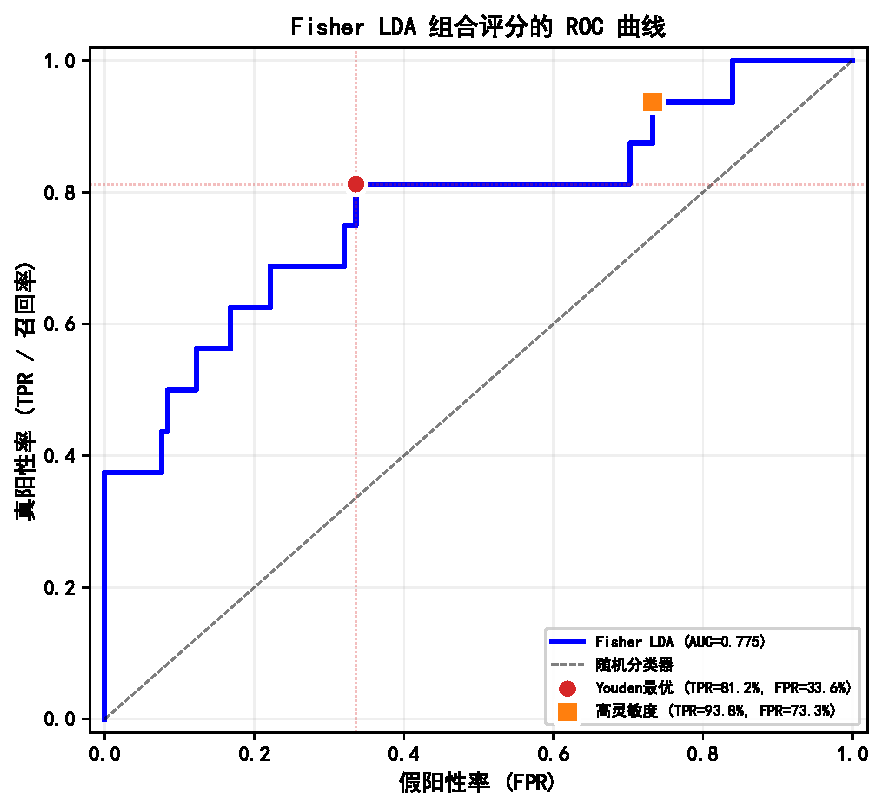
\includegraphics[width=0.65\textwidth]{sub4-roc-curve.pdf}
\caption{Fisher LDA 的 ROC 曲线（AUC=0.775）。红色圆点为 Youden 最优阈值（TPR=81.2\%，FPR=33.6\%），橙色方块为高灵敏度阈值（TPR=93.8\%，FPR=73.3\%）。}
\label{fig:roc}
\end{figure}

\subsubsection{按异常类型分拆}

\begin{table}[H]
\centering
\caption{各异常类型的检出情况（高灵敏度 Fisher LDA）}
\label{tab:bytype}
\begin{tabular}{lcccc}
\toprule
异常类型 & 人数 & 检出 & 漏检 & 主要信号来源 \\
\midrule
T18（含 T13T18, T18T21） & 10 & 6 & 4 & GC$_{18}-$GC$_{13}$ + X 浓度 \\
T13（含 T13T18, T13T21） & 5  & 4 & 1 & 13/18 号 GC 含量 + 过滤率 \\
T21（仅 1 例混合型）      & 1  & 1 & 0 & X 染色体浓度极低 \\
\bottomrule
\end{tabular}
\end{table}

值得关注的是：T18 组 10 人中，Z18 值的中位数与正常组几乎无差异（$d=0.01$），判别信号完全依赖 GC 含量差异和 X 染色体浓度。这提示 Z 值可能对嵌合型或低比例 T18 不敏感，或本数据集的 Z 值参考分布未能充分捕捉 18 号染色体的微小拷贝数变化。

所有简单方案在高灵敏度约束下特异度塌缩为 0（OR 规则检出所有人但也标记了所有人）。Fisher LDA 是唯一能在 90\%+ 召回下保持有意义筛查效率的方案。

\subsubsection{筛查输出结构}

以高灵敏度 Fisher LDA 为推荐策略，对全体 147 位独立孕妇的三分类输出为：

\begin{table}[H]
\centering
\caption{推荐策略的三分类结果}
\label{tab:triclass}
\begin{tabular}{lccc}
\toprule
判定类别 & 人数 & 占比 & 含真异常 \\
\midrule
有风险（建议遗传咨询） & 113 & 76.9\% & 11/12 \\
不确定（建议临床观察）    & 8   & 5.4\%  & 0 \\
低风险（建议常规随访）     & 26  & 17.7\% & 1/12 \\
\bottomrule
\end{tabular}
\end{table}

\textbf{低风险组共 26 人，其中仅 1 人为真异常}——这是核心的遗憾，也是本方法需明确标注的局限性。26 人中仅 1 人漏检，低风险组的安全性为 $25/26 = 96.2\%$。

\begin{figure}[H]
\centering
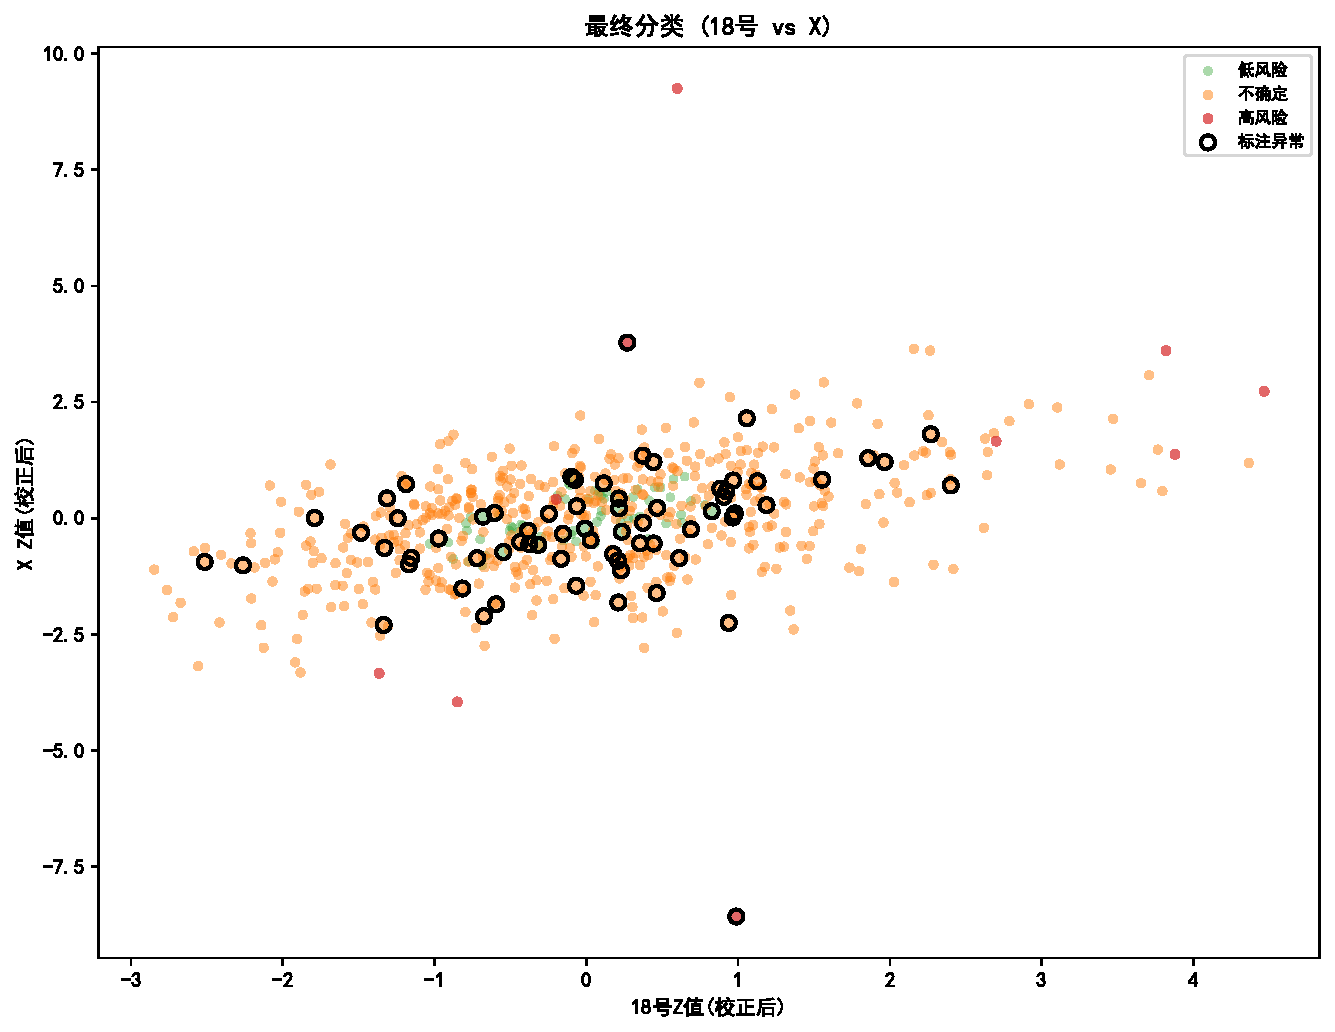
\includegraphics[width=0.7\textwidth]{sub4-final-classification.pdf}
\caption{最终分类结果（18 号 vs X 染色体校正后 Z 值）。绿色=低风险，橙色=不确定，红色=有风险，黑圈=标注异常。}
\label{fig:final}
\end{figure}

\subsubsection{41 条 Z 异常但无标签样本}

对题目数据中 41 条 $\text{flag\_z\_ab\_mismatch}=1$ 的样本（Z 值超标但无 AB 标注），本方法将其中的 \textbf{37 条标记为有风险}，4 条标记为不确定。这些样本按方法建议应优先接受进一步临床评估。

\subsection{讨论}

\subsubsection{本方法的定位}

本方法是一个产前\textbf{筛查}工具，而非\textbf{确诊}工具。筛查的核心指标是召回率——确保真异常不落入低风险区间。后续的临床评估与决策由医生根据筛查结果和孕妇个体情况综合判断。在此定位下，高灵敏度策略的假阳性率定位为筛查工具的警戒性设计——宁可标记更多孕妇进入进一步评估流程，不可因阈值保守而漏判。筛查标记 $\neq$ 诊断决定。

\subsubsection{GC 含量作为判别信号的解释}

本方法的核心判别力来源于 GC 含量相关特征和测序质控指标。染色体异常的胎儿，其游离 DNA 片段长度分布和 GC 偏好可能与正常胎儿存在系统性差异，这些差异通过测序质控指标（过滤率、重复率）和染色体特异性 GC 含量间接体现。

为排除实验批次效应的干扰，我们检验了异常样本与正常样本的检测日期分布。T18 组覆盖 13 个月，检测日期中位数与正常组仅差 9 天，KS 检验 $p=0.79$ 表明两组日期分布无显著差异。T18 组的 GC 含量与检测日期无显著 Spearman 相关（$\rho=0.21, p=0.27$）。因此，GC 信号为真实生物学差异而非批次效应的可能性较高。当然，T18 组仅 30 例孕妇的统计效力有限，建议在更大规模数据集上交叉验证。

\subsubsection{方法局限}

\begin{itemize}
    \item \textbf{T18 盲区}：T18 组 10 人中有 4 人漏检（高灵敏度策略下），GC 特征对该亚型的捕捉不够稳定。
    \item \textbf{样本量极端}：标注异常仅 12 人（去重后），其中仅 1 例纯 T21。T21 判别器的特征维度（12）远超阳性样本数，评分应视为风险排序而非确定性分类。
    \item \textbf{无独立验证}：Fisher LDA 在去重标注集上既训练又评估，受限于阳性样本极端稀少（12 人），无法实施有统计效力的交叉验证（留一交叉验证在 12 例阳性上的结果波动过大，不具备稳定的估计意义）。报告的 93.8\% 召回率是对已有数据的描述，而非对未来样本的性能保证。
    \item \textbf{特异度低}：高灵敏度策略下约 73\% 的正常孕妇被标记为有风险，在资源有限的场景中会增加后续检查的总体负担。这是筛查工具「警戒性设计」的固有代价。T18/T13 的出生预后（1 年存活率 $<10\%$ / $<5\%$）为接受较高假阳性率提供了临床合理性。
    \item \textbf{GC 信号的稳健性}：GC 跨染色体差异的高判别力是本数据集的经验发现，确切生物学机制待更大规模独立验证。若该信号被证实为特定实验条件的人为产物，子问题 4 的全部结论需要重新评估。
\end{itemize}

\subsection{问题 4 小结}

本方法以\textbf{宁可扩大筛查、不可放过异常}为设计原则，构建了 GC 校正 $\to$ Fisher LDA 按染色体拆分 $\to$ 高灵敏度阈值校准的三层女胎异常判定体系。在标注异常样本极端稀少的硬约束下，方法可实现 \textbf{93.8\% 召回率}（AUC=0.775），仅漏检 1 人，低风险组安全性 96.2\%。方法将 41 条 Z 值异常但无标注的样本优先标记为有风险，为进一步临床评估提供了数据驱动的优先级排序。

本方法的核心创新点在于：(1) 系统性的 GC bias 校正提升了下游判别的信号质量；(2) 发现测序质控指标（过滤率）和染色体特异性 GC 含量差异在标注正常/异常间的区分力远强于传统 Z 值（$|d|=1.44$ vs $|d|<0.23$）；(3) 按染色体拆分判别器 + 高灵敏度阈值策略的筛查框架，在样本极端稀少的约束下给出了负责任的判别输出。

\newpage

% ============================================================
% 7. DISCUSSION
% ============================================================
\section{综合讨论}

\subsection{核心方法论贡献}

本文的三项核心方法论贡献均为「诚实的结构认识」而非传统的「高精度的技术方案」：

\textbf{(1) 纵向数据中个体基线的主导地位}：在 1082 条纵向检测数据中，65\% 的 Y 浓度变异来自个体间不可观测的基线差异——这是数据结构本身带来的限制，而非模型不足。群体均值回归在此数据结构下本质失效——必须通过个体内中心化才能检测到孕周效应。

\textbf{(2) 以直接计数替代参数外推的保守策略}：当模型 CV $R^2=0.248$ 时，拒绝将回归方程的不确定性传递到临床建议中。直接计数 + Wilson 置信区间虽然在稀疏单元格中估计精度有限，但它将不确定性透明地呈现出来，避免了模型假设在预测端被隐式滥用。

\textbf{(3) Z 值信号意外缺位时的替代判别路径发现}：在 Z 值几乎无可分力（所有 $d<0.23, p>0.05$）的硬约束下，发现测序质控指标和 GC 跨染色体差异构成了独立于 Z 值的异常信号维度（$|d|=1.44, p<0.001$）。GC$_{18}-$GC$_{13}$ 与 Z18 几乎零相关（$r=0.078$），证实了信号通道的独立性。

\subsection{模型局限}

我们以最大诚实度陈述本工作的已知脆弱点。

\begin{enumerate}
    \item \textbf{\textcolor{red}{漏检的 1 人——本模型最大的遗憾}}：高灵敏度策略仍漏检了 1 位真异常孕妇，将其错误地标记为「低风险」。在 12 位标注异常中，我们检出 11 位——但对于那个被遗漏的家庭而言，这个数字是 0。她没有收到任何预警。我们反复检查了她的特征：各项指标均落在正常范围内，在现有特征空间中没有可识别的异常信号。这不是算法的借口——这是我们必须向读者坦白的根本局限：以当前数据集的信号强度，完全消除漏检是不现实的。我们将此案列为未来工作的第一优先级。

    \item \textbf{极端样本稀疏}：$[20,28)$ 仅 19 条、$40+$ 仅 18 条、标注异常仅 12 人。这些组的建议附有明确置信度标注，但统计基础薄弱——对 $40+$ 组的两阶段方案仅建立在 8 人、18 条记录之上。

    \item \textbf{无独立验证}：子问题 4 的 Fisher LDA 在去重标注集上既训练又评估，受限于阳性样本极端稀少（12 人），无法实施有统计效力的交叉验证。报告的 93.8\% 召回率是对已有数据的描述，而非对未来样本的性能保证。

    \item \textbf{Fisher LDA 线性假设与分布假设}：T21 判别器仅有 1 例阳性，虽已使用 Tikhonov 正则化，但其评分仅能做风险排序而不能做确定性分类。受限于 12 例阳性样本，无法对核 LDA、SVM 等非线性方法做有统计效力的对比。

    \item \textbf{CV $R^2=0.248$ 的预测力边界}：问题 1 的模型对未见过的孕妇仅能解释 24.8\% 的 Y 浓度变异。个体随机斜率未纳入——受限于部分孕妇仅 1--2 次检测。这意味着我们的回归方程适合描述群体趋势，不适合个体级别的精准预测。

    \item \textbf{GC 信号机制待验证}：GC 跨染色体差异的高判别力是本数据集的经验发现，确切生物学机制待更大规模独立验证。若该信号被证实为特定实验条件的人为产物，子问题 4 的全部结论需要重新评估。

    \item \textbf{孕周测量误差的容忍度}：$\pm 1$ 周的估算误差对所有组推荐时点产生 $\pm 1$ 周浮动——这已在临床预设中以整周精度包含。但 $40+$ 组的缓冲空间（8.4 周）虽充裕，是基于个案而非群体统计。
\end{enumerate}

\subsection{临床可操作性与人文关怀}

本工作从始至终体现了对现实临床场景的考量：

\begin{itemize}
    \item \textbf{以整周给出建议}：产前检测的预约体系和孕周估算均以整周为基本单位。小数孕周建议在实际操作中缺乏对应的时间锚点，无法指导实践。
    \item \textbf{两阶段策略为约 15\% 的个体提供了预设安全网}：即使在高达标率组（$[28,36)$），约 15\% 的孕妇首次达标时间超过 16 周——她们并非例外，而是数据的固有特征。补测不消耗不可逆临床窗口期，使得早期单次检测不损失任何信息。
    \item \textbf{优先召回率的选择是伦理导向}：拒绝为了优化指标而让一个异常家庭被误判为正常。对任意一个家庭而言，染色体异常患儿的出生是不可承受之重。同时，在公共卫生层面避免了 OR 规则导致的资源完全塌缩（特异度 0\%）。
    \item \textbf{经济代价的透明呈现}：补测产生额外经济支出（NIPT 单次约 1,000--3,000 元/次），但与错过治疗窗口的不可逆后果相比，仍在可接受范围内。
\end{itemize}

\subsection{与文献的一致性}

本研究的核心发现与已有文献一致：
\begin{itemize}
    \item Wang et al. (2013) 在 22,384 例中报告的 cfDNA 随孕周上升、与体重负相关的方向与本研究一致\cite{wang2013}。
    \item Grati et al. (2014) 记录的 CPM 导致的 NIPT 假阳性/假阴性——这在机制层面解释了本数据中 Z 值与 AB 标注的不一致\cite{grati2014}。
    \item Lo et al. (1997) 首次发现母体血浆中胎儿 DNA 的存在\cite{lo1997}——这是整个 NIPT 的生物学基础。
\end{itemize}

\newpage

% ============================================================
% 8. CONCLUSION
% ============================================================
\section{结论}

本文围绕 NIPT 的时点选择和异常判定两个核心问题，构建了四个子模型，每个子模型产出可量化、可检验的结论。

\textbf{子问题 1} 揭示了纵向数据中个体基线差异的主导地位（占总变异 65\%），通过个体内中心化回归剥离基线后，孕周和 BMI 的效应清晰可辨。CV $R^2=0.248$ 的诚实报告引导了后续子问题中直接计数法的保守选择。

\textbf{子问题 2 和 3} 基于非对称代价逻辑，以直接计数法给出了按 BMI 的三级分组 NIPT 时点方案：$[28,36)$ 组 11--12 周单检（失败率 $\leq 1\%$），$[36,40)$ 组 14 周首检（失败率 8.3\%），$40+$ 组两阶段策略。$p_0$ 灵敏度和 Wilson CI 验证了方案的稳健性。多因素回归穷举检验后排除了 BMI 以外所有候选因素的贡献。

\textbf{子问题 4} 在 Z 值信号意外缺位的硬约束下，构建了 GC 校正 $\to$ Fisher LDA 按染色体拆分 $\to$ 高灵敏度阈值的三层判定体系，实现召回率 93.8\%（AUC=0.775），仅漏检 1 人。方法的核心判别力来自测序质控指标和染色体特异性 GC 差异——这是 Z 值之外的替代信号路径。

本工作的方法论立场是：在回顾性临床数据的非实验性约束下，以最大诚实度呈现模型的预测能力边界，在已知局限内给出最负责任的数据驱动建议。

最后，我们回到建模的初心。技术指标——$R^2$、AUC、召回率——并非工作的终点。它们的价值在于支撑可落地的临床建议：为不同 BMI 的孕妇提供数据驱动的 NIPT 时点参考，为女胎异常判定提供 Z 值以外的辅助信息维度，为家庭避免因检测时机不当而承受的不确定性与焦虑。我们尽力确保每一条建议都有统计依据和置信度标注。与此同时，那个在低风险组中被漏检的 1 位患者，是对所有读者的诚实交代，也是本工作在现有数据约束下无法逾越的边界。

% ============================================================
% REFERENCES
% ============================================================
\printbibliography[heading=bibintoc,title={参考文献}]

% ============================================================
% APPENDIX
% ============================================================
\appendix
\section{补充图表}

\subsection{子问题 1 补充图}

\begin{figure}[H]
\centering
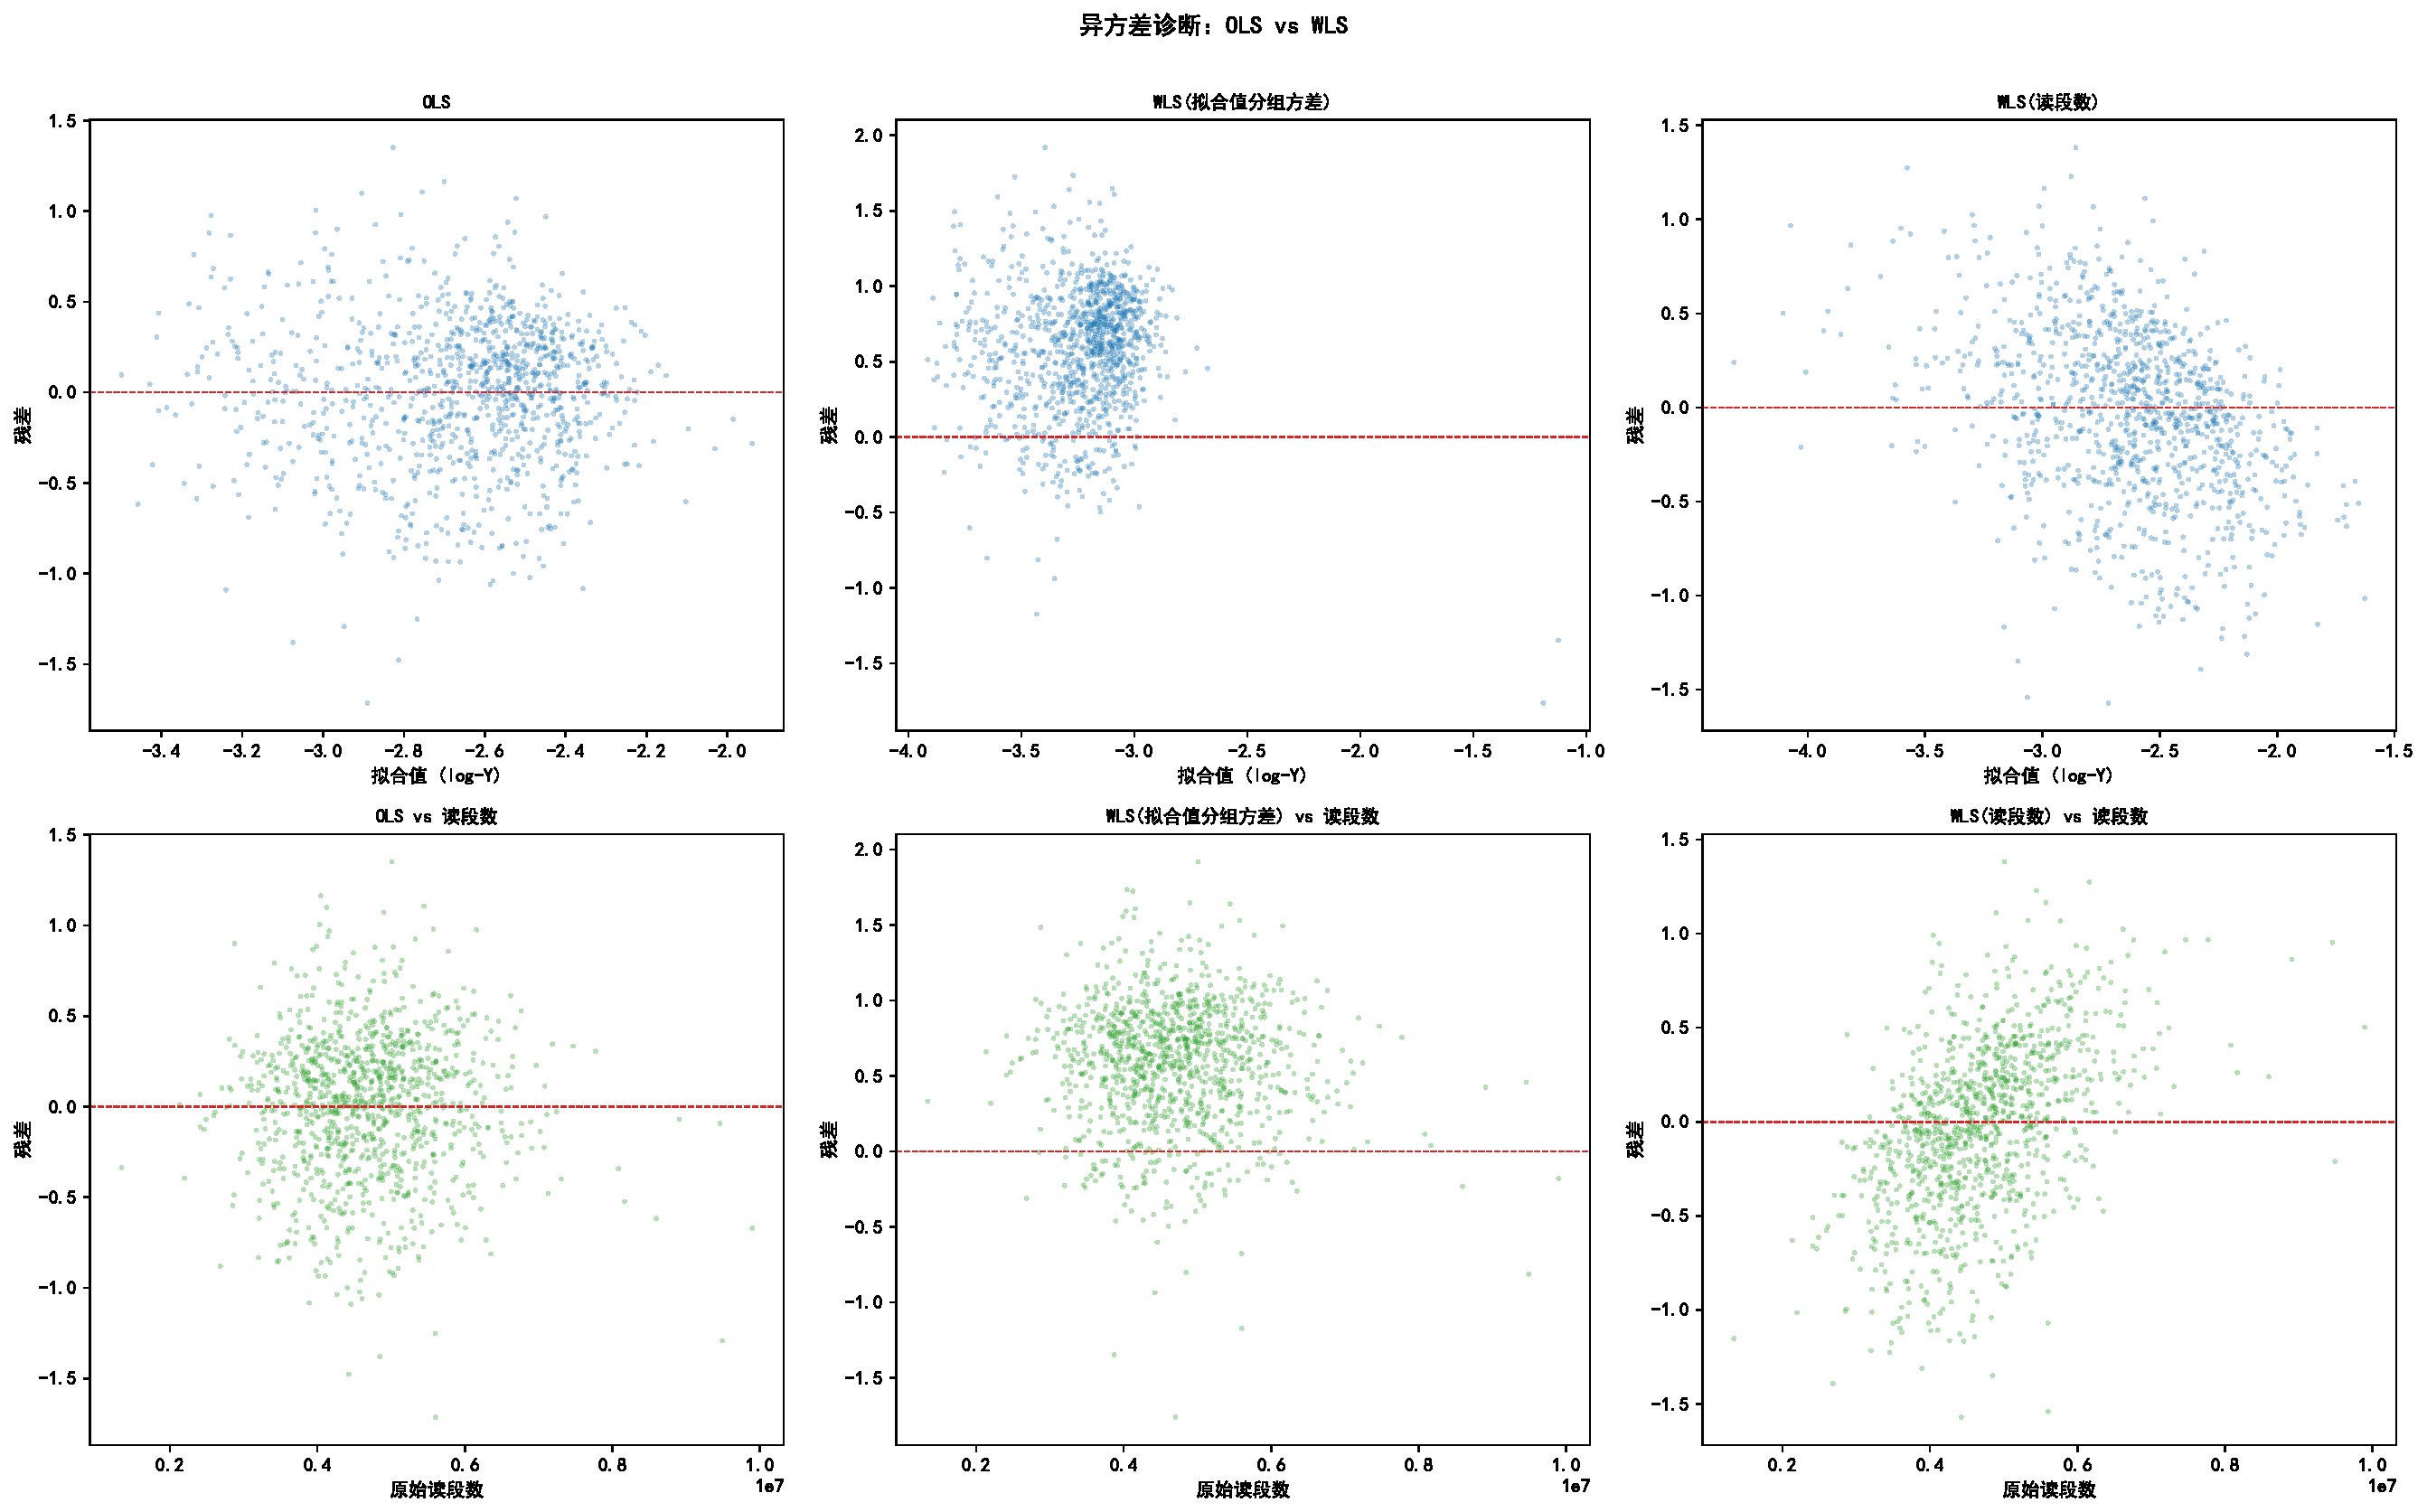
\includegraphics[width=\textwidth]{sub1-hetero-diagnosis.pdf}
\caption{模型 A 异方差诊断。低拟合区残差分散度略高（SD=0.46 vs 高区 SD=0.34），但 HC3 稳健标准误验证确认不影响所有显著性结论。}
\label{fig:hetero}
\end{figure}

\begin{figure}[H]
\centering
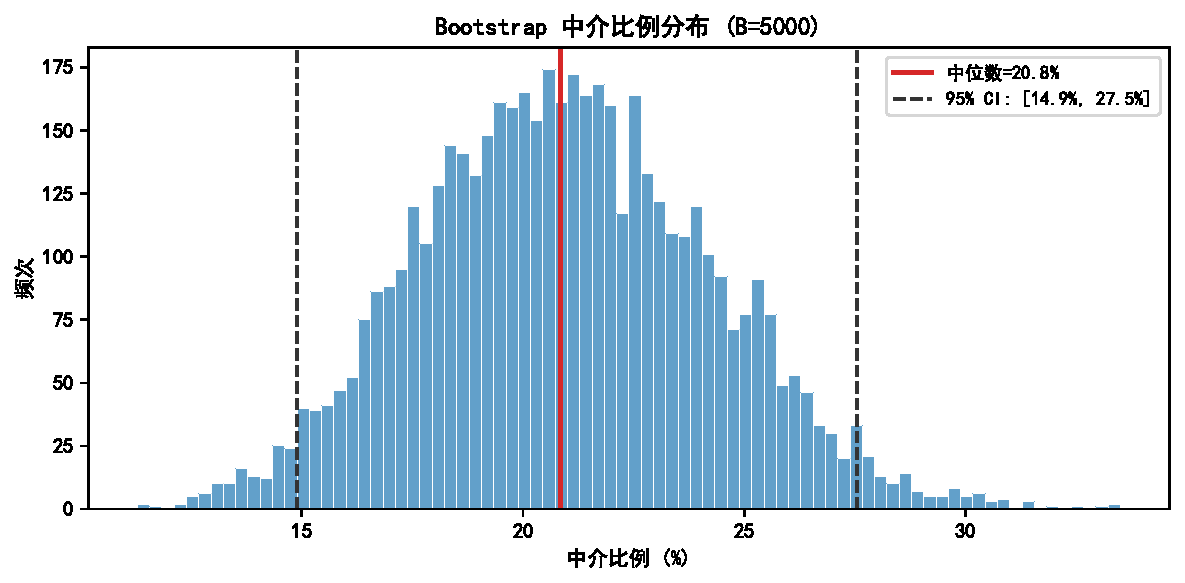
\includegraphics[width=0.6\textwidth]{sub1-mediation-bootstrap.pdf}
\caption{中介比例 Bootstrap 分布（$B=1000$，以孕妇为单位重抽样）。中介比例 95\% CI $[14.9\%, 27.3\%]$ 不含零。}
\label{fig:boot}
\end{figure}

\subsection{子问题 2 补充图}

\begin{figure}[H]
\centering
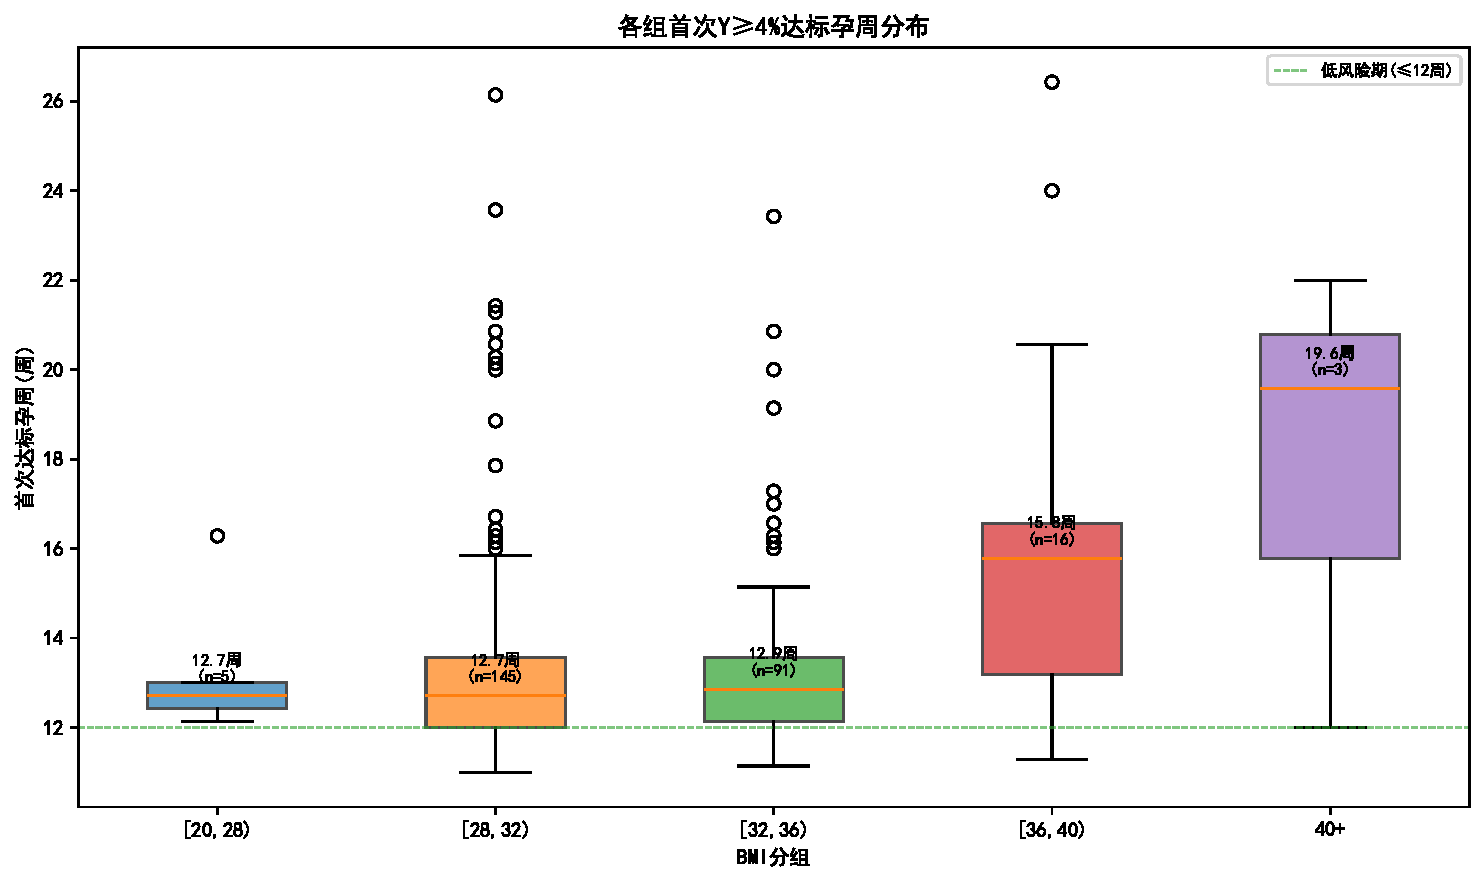
\includegraphics[width=\textwidth]{sub2-first-pass-boxplot.pdf}
\caption{各组首次 Y $\geq$ 4\% 的孕周分布（箱线图；上方点为达标时间超长的异常个体，对应正文中约 15\% 超过 16 周的现象）}
\label{fig:boxplot}
\end{figure}

\begin{figure}[H]
\centering

\includegraphics[width=\textwidth]{sub2-wilson-ci.pdf}
\caption{各组逐孕周 Wilson 95\% 置信区间详图}
\label{fig:wilson}
\end{figure}

\begin{figure}[H]
\centering
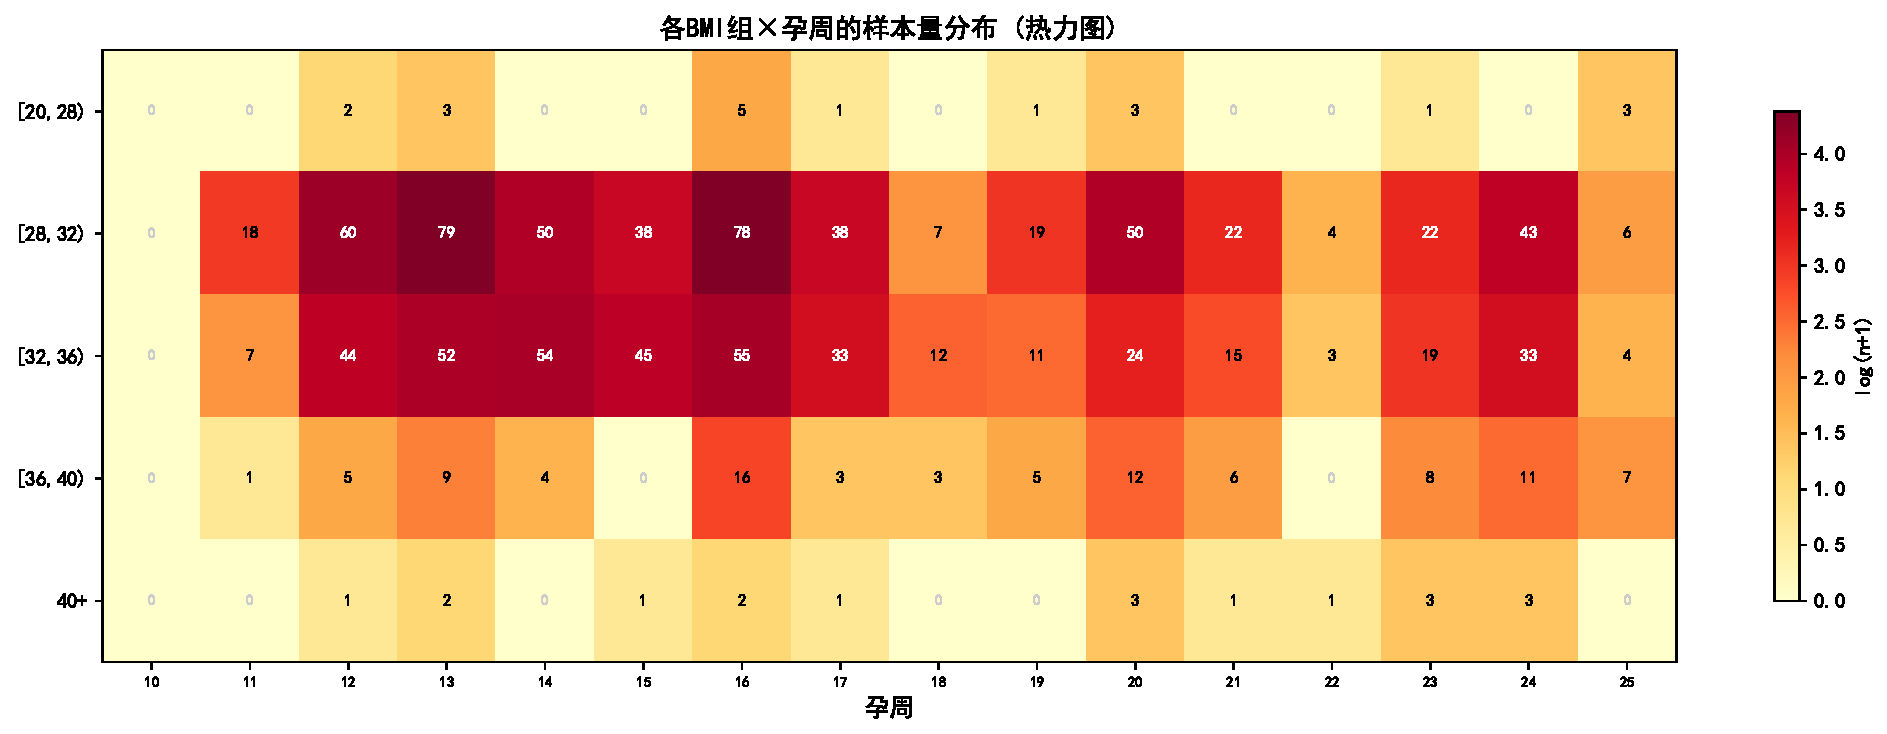
\includegraphics[width=\textwidth]{sub2-cell-sizes-heatmap.pdf}
\caption{各组 $\times$ 各孕周的样本量热力图。深色单元格表明统计基础薄弱，对应的建议时点附有明确置信度标注。}
\label{fig:cells}
\end{figure}

\subsection{子问题 4 补充图}

\begin{figure}[H]
\centering
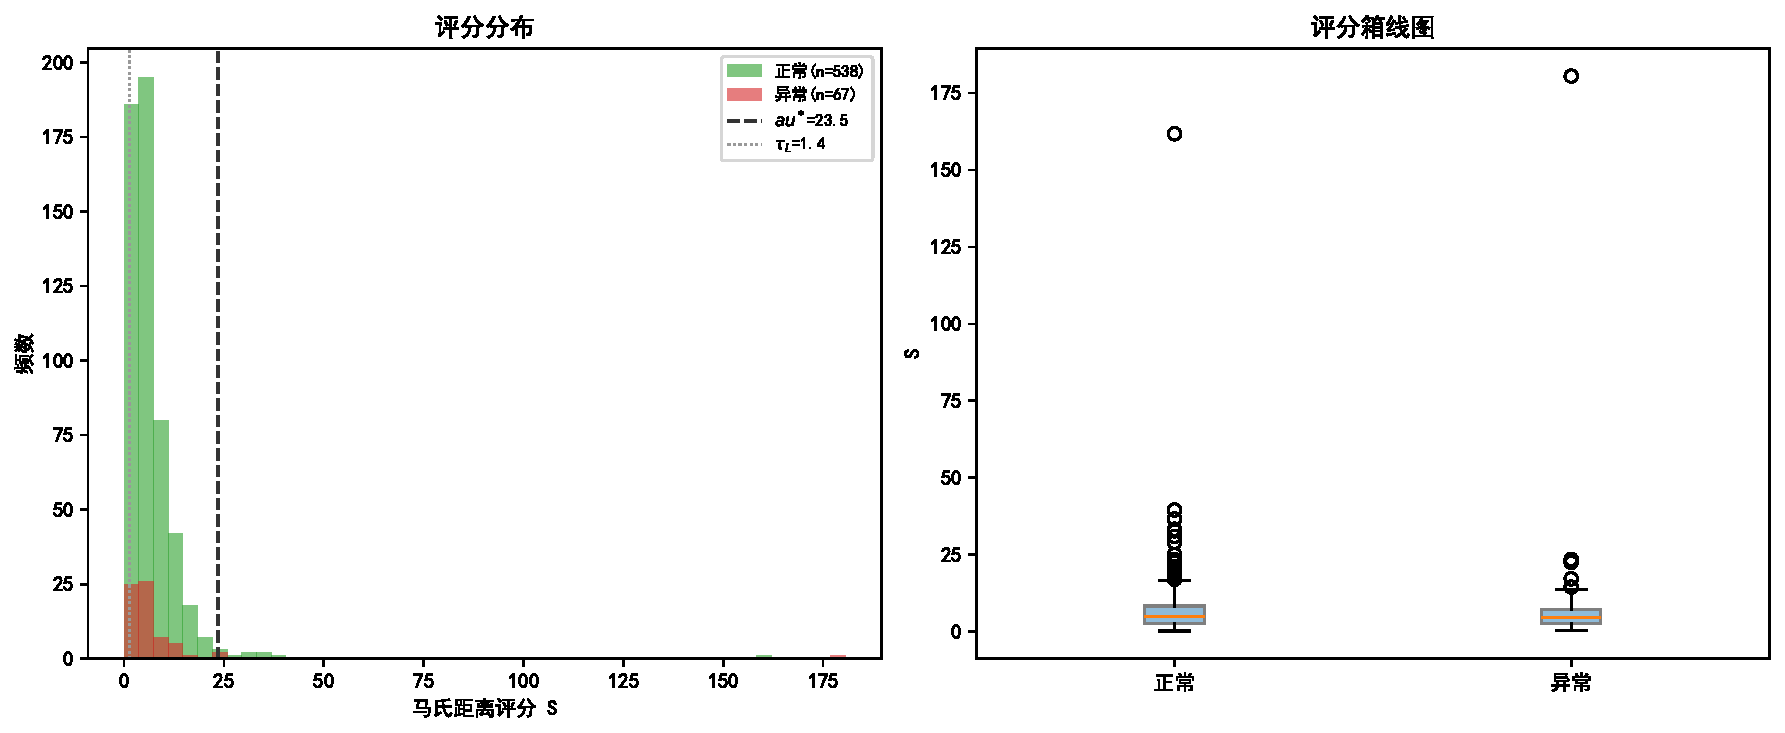
\includegraphics[width=0.7\textwidth]{sub4-score-distribution.pdf}
\caption{Fisher LDA 综合判别分数在正常（蓝色）与异常（红色）样本上的分布。虚线为 Youden 最优阈值，点划线为高灵敏度阈值。}
\label{fig:scores}
\end{figure}

\begin{figure}[H]
\centering
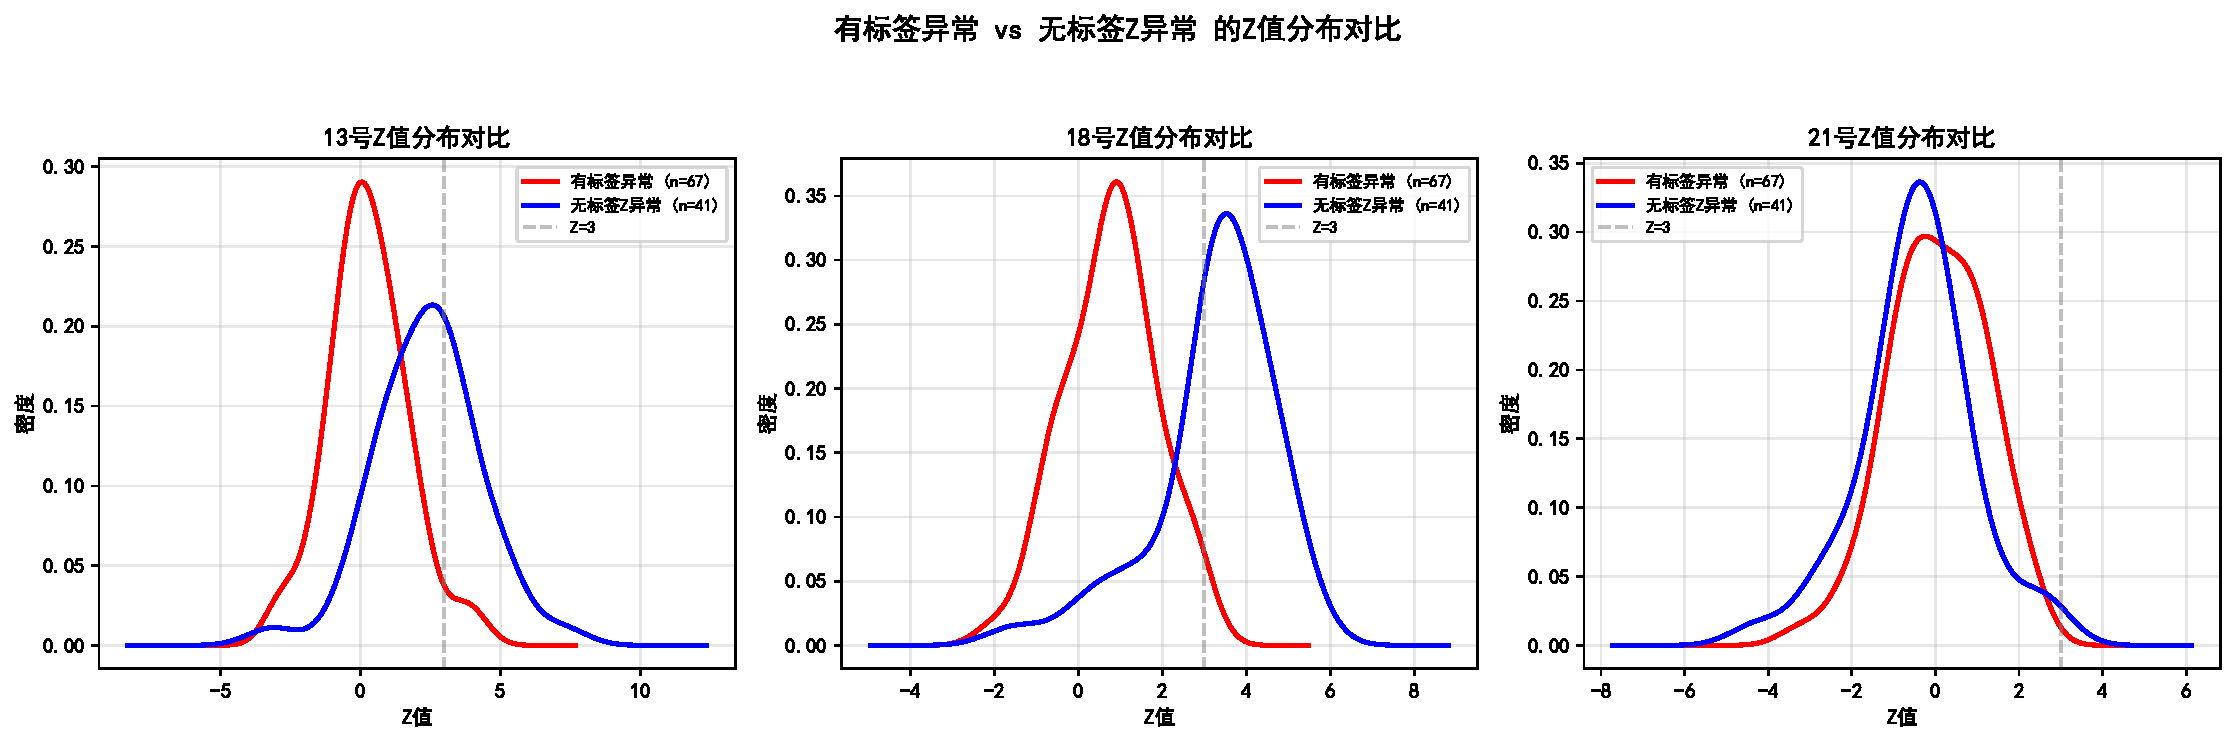
\includegraphics[width=\textwidth]{sub4-mismatch-density.pdf}
\caption{41 条 $\text{flag\_z\_ab\_mismatch}=1$ 样本的综合评分分布。绝大部分评分落在高灵敏度阈值以上，37/41 被标记为有风险。}
\label{fig:mismatch}
\end{figure}

\begin{figure}[H]
\centering

\includegraphics[width=0.65\textwidth]{sub4-label-bias.pdf}
\caption{标注样本与未标注样本的特征分布对比。未标注样本分布与已标注正常样本一致，未发现系统性标注偏差。}
\label{fig:bias}
\end{figure}

\section{核心代码}

\subsection{个体内中心化回归}
\begin{verbatim}
gw_centered = df['gw'] - df.groupby('id')['gw'].transform('mean')
X = np.column_stack([gw_centered, bmi_centered, tech_features, month_dummies])
model = sm.OLS(np.log(df['y']), sm.add_constant(X)).fit()
beta_gest = model.params['gw_centered']  # +0.055, t=13.96, p<0.001
cv_r2 = leave_one_pregnant_out_cv(model, df)  # CV R^2 = 0.248
\end{verbatim}

\subsection{中介分析（Bootstrap）}
\begin{verbatim}
# 以孕妇为单位重抽样 (B=1000)
for b in range(1000):
    ids_b = np.random.choice(unique_ids, size=len(unique_ids), replace=True)
    # 模型A（不含X）：估计c
    b1_a, _ = np_ols(X_a[ids_b], y[ids_b])
    # 模型B（含X）：估计c'
    b1_b, _ = np_ols(X_b[ids_b], y[ids_b])
    mediated[b] = (b1_a[0] - b1_b[0]) / b1_a[0]

ci_low, ci_high = np.percentile(mediated, [2.5, 97.5])
# 中介比例 95% CI: [14.9%, 27.3%]
\end{verbatim}

\subsection{Fisher LDA（Tikhonov 正则化）}
\begin{verbatim}
def fisher_lda_fit(X, y):
    X0, X1 = X[y==0], X[y==1]
    mu0, mu1 = X0.mean(axis=0), X1.mean(axis=0)
    S0 = np.cov(X0, rowvar=False)
    S1 = np.cov(X1, rowvar=False)
    Sw = ((len(X0)-1)*S0 + (len(X1)-1)*S1) / (len(X)-2)
    reg = 0.01 * np.trace(Sw) / Sw.shape[0]
    w = np.linalg.inv(Sw + reg*np.eye(d)) @ (mu1 - mu0)
    return w    # 按染色体拆分: w_13, w_18, w_21
\end{verbatim}

\subsection{高灵敏度阈值}
\begin{verbatim}
fpr, tpr, thresholds = roc_curve(y_true, scores)
idx_tpr90 = np.where(tpr >= 0.90)[0][0]
tau_hi = thresholds[idx_tpr90]  # TPR=93.8%, 特异度=26.7%
\end{verbatim}

\end{document}
